%%%%%%%%%%%%%%%%%%%%%%%%%%%%%%%%%%%%%%%%
% datoteka diploma-FRI-vzorec.tex
%
% vzorčna datoteka za pisanje diplomskega dela v formatu LaTeX
% na UL Fakulteti za računalništvo in informatiko
%
% na osnovi starejših verzij vkup spravil Franc Solina, maj 2021
% prvo verzijo je leta 2010 pripravil Gašper Fijavž
%
% za upravljanje z literaturo ta vezija uporablja BibLaTeX
%
% svetujemo uporabo Overleaf.com - na tej spletni implementaciji LaTeXa ta vzorec zagotovo pravilno deluje
%

\documentclass[a4paper,12pt,openright]{book}
%\documentclass[a4paper, 12pt, openright, draft]{book}  Nalogo preverite tudi z opcijo draft, ki pokaže, katere vrstice so predolge! Pozor, v draft opciji, se slike ne pokažejo!
\usepackage{float}

\usepackage[utf8]{inputenc}   % omogoča uporabo slovenskih črk kodiranih v formatu UTF-8
\usepackage[slovene,english]{babel}    % naloži, med drugim, slovenske delilne vzorce
\usepackage[pdftex]{graphicx}  % omogoča vlaganje slik različnih formatov
\usepackage{fancyhdr}          % poskrbi, na primer, za glave strani
\usepackage{amssymb}           % dodatni matematični simboli
\usepackage{amsmath}           % eqref, npr.
\usepackage{hyperxmp}
\usepackage[hyphens]{url}
\usepackage{csquotes}
\usepackage[pdftex, colorlinks=true,
						citecolor=black, filecolor=black, 
						linkcolor=black, urlcolor=black,
						pdfproducer={LaTeX}, pdfcreator={LaTeX}]{hyperref}

\usepackage{color}
\usepackage{soul}
\usepackage{multirow} 


\usepackage[
backend=biber,
style=numeric,
sorting=nty,
]{biblatex}


\addbibresource{literatura.bib} %Imports bibliography file


%%%%%%%%%%%%%%%%%%%%%%%%%%%%%%%%%%%%%%%%
%	DIPLOMA INFO
%%%%%%%%%%%%%%%%%%%%%%%%%%%%%%%%%%%%%%%%
\newcommand{\ttitle}{Ocena kakovosti ponarejenih posnetkov}
\newcommand{\ttitleEn}{Visual Realism Assessment of Deepfakes}
\newcommand{\tsubject}{\ttitle}
\newcommand{\tsubjectEn}{\ttitleEn}
\newcommand{\tauthor}{Luka Dragar}
\newcommand{\tkeywords}{globoki ponaredek,vizualni realizem}
\newcommand{\tkeywordsEn}{deepfake,visual realism}

%%%%%%%%%%%%%%%%%%%%%%%%%%%%%%%%%%%%%%%%
%	HYPERREF SETUP
%%%%%%%%%%%%%%%%%%%%%%%%%%%%%%%%%%%%%%%%
\hypersetup{pdftitle={\ttitle}}
\hypersetup{pdfsubject=\ttitleEn}
\hypersetup{pdfauthor={\tauthor}}
\hypersetup{pdfkeywords=\tkeywordsEn}

%%%%%%%%%%%%%%%%%%%%%%%%%%%%%%%%%%%%%%%%
% postavitev strani
%%%%%%%%%%%%%%%%%%%%%%%%%%%%%%%%%%%%%%%%  

\addtolength{\marginparwidth}{-20pt} % robovi za tisk
\addtolength{\oddsidemargin}{40pt}
\addtolength{\evensidemargin}{-40pt}

\renewcommand{\baselinestretch}{1.3} % ustrezen razmik med vrsticami
\setlength{\headheight}{15pt}        % potreben prostor na vrhu
\renewcommand{\chaptermark}[1]%
{\markboth{\MakeUppercase{\thechapter.\ #1}}{}} \renewcommand{\sectionmark}[1]%
{\markright{\MakeUppercase{\thesection.\ #1}}} \renewcommand{\headrulewidth}{0.5pt} \renewcommand{\footrulewidth}{0pt}
\fancyhf{}
\fancyhead[LE,RO]{\sl \thepage} 
%\fancyhead[LO]{\sl \rightmark} \fancyhead[RE]{\sl \leftmark}
\fancyhead[RE]{\sc \tauthor}              % dodal Solina
\fancyhead[LO]{\sc Diplomska naloga}     % dodal Solina


\newcommand{\BibLaTeX}{{\sc Bib}\LaTeX}
\newcommand{\BibTeX}{{\sc Bib}\TeX}

%%%%%%%%%%%%%%%%%%%%%%%%%%%%%%%%%%%%%%%%
% naslovi
%%%%%%%%%%%%%%%%%%%%%%%%%%%%%%%%%%%%%%%%  

\newcommand{\autfont}{\Large}
\newcommand{\titfont}{\LARGE\bf}
\newcommand{\clearemptydoublepage}{\newpage{\pagestyle{empty}\cleardoublepage}}
\setcounter{tocdepth}{1}	      % globina kazala

%%%%%%%%%%%%%%%%%%%%%%%%%%%%%%%%%%%%%%%%
% konstrukti
%%%%%%%%%%%%%%%%%%%%%%%%%%%%%%%%%%%%%%%%  
\newtheorem{izrek}{Izrek}[chapter]
\newtheorem{trditev}{Trditev}[izrek]
\newenvironment{dokaz}{\emph{Dokaz.}\ }{\hspace{\fill}{$\Box$}}


%%%%%%%%%%%%%%%%%%%%%%%%%%%%%%%%%%%%%%%%%%%%%%%%%%%%%%%%%%%%%%%%%%%%%%%%%%%%%%%
%% PDF-A
%%%%%%%%%%%%%%%%%%%%%%%%%%%%%%%%%%%%%%%%%%%%%%%%%%%%%%%%%%%%%%%%%%%%%%%%%%%%%%%

%%%%%%%%%%%%%%%%%%%%%%%%%%%%%%%%%%%%%%%% 
% define medatata
%%%%%%%%%%%%%%%%%%%%%%%%%%%%%%%%%%%%%%%% 
\def\Title{\ttitle}
\def\Author{\tauthor, matjaz.kralj@fri.uni-lj.si}
\def\Subject{\ttitleEn}
\def\Keywords{\tkeywordsEn}

%%%%%%%%%%%%%%%%%%%%%%%%%%%%%%%%%%%%%%%% 
% \convertDate converts D:20080419103507+02'00' to 2008-04-19T10:35:07+02:00
%%%%%%%%%%%%%%%%%%%%%%%%%%%%%%%%%%%%%%%% 
\def\convertDate{%
    \getYear
}

{\catcode`\D=12
 \gdef\getYear D:#1#2#3#4{\edef\xYear{#1#2#3#4}\getMonth}
}
\def\getMonth#1#2{\edef\xMonth{#1#2}\getDay}
\def\getDay#1#2{\edef\xDay{#1#2}\getHour}
\def\getHour#1#2{\edef\xHour{#1#2}\getMin}
\def\getMin#1#2{\edef\xMin{#1#2}\getSec}
\def\getSec#1#2{\edef\xSec{#1#2}\getTZh}
\def\getTZh +#1#2{\edef\xTZh{#1#2}\getTZm}
\def\getTZm '#1#2'{%
    \edef\xTZm{#1#2}%
    \edef\convDate{\xYear-\xMonth-\xDay T\xHour:\xMin:\xSec+\xTZh:\xTZm}%
}

%\expandafter\convertDate\pdfcreationdate 

%%%%%%%%%%%%%%%%%%%%%%%%%%%%%%%%%%%%%%%%
% get pdftex version string
%%%%%%%%%%%%%%%%%%%%%%%%%%%%%%%%%%%%%%%% 
\newcount\countA
\countA=\pdftexversion
\advance \countA by -100
\def\pdftexVersionStr{pdfTeX-1.\the\countA.\pdftexrevision}


%%%%%%%%%%%%%%%%%%%%%%%%%%%%%%%%%%%%%%%%
% XMP data
%%%%%%%%%%%%%%%%%%%%%%%%%%%%%%%%%%%%%%%%  
\usepackage{xmpincl}
%\includexmp{pdfa-1b}

%%%%%%%%%%%%%%%%%%%%%%%%%%%%%%%%%%%%%%%%
% pdfInfo
%%%%%%%%%%%%%%%%%%%%%%%%%%%%%%%%%%%%%%%%  
\pdfinfo{%
    /Title    (\ttitle)
    /Author   (\tauthor, luka.dragar2@gmail.com)
    /Subject  (\ttitleEn)
    /Keywords (\tkeywordsEn)
    /ModDate  (\pdfcreationdate)
    /Trapped  /False
}

%%%%%%%%%%%%%%%%%%%%%%%%%%%%%%%%%%%%%%%%
% znaki za copyright stran
%%%%%%%%%%%%%%%%%%%%%%%%%%%%%%%%%%%%%%%%  

\newcommand{\CcImageCc}[1]{%
	\includegraphics[scale=#1]{cc_cc_30.pdf}%
}
\newcommand{\CcImageBy}[1]{%
	\includegraphics[scale=#1]{cc_by_30.pdf}%
}
\newcommand{\CcImageSa}[1]{%
	\includegraphics[scale=#1]{cc_sa_30.pdf}%
}

%%%%%%%%%%%%%%%%%%%%%%%%%%%%%%%%%%%%%%%%%%%%%%%%%%%%%%%%%%%%%%%%%%%%%%%%%%%%%%%
%%%%%%%%%%%%%%%%%%%%%%%%%%%%%%%%%%%%%%%%%%%%%%%%%%%%%%%%%%%%%%%%%%%%%%%%%%%%%%%

\begin{document}
\selectlanguage{english}
\frontmatter
\setcounter{page}{1} %
\renewcommand{\thepage}{}       % preprečimo težave s številkami strani v kazalu

%%%%%%%%%%%%%%%%%%%%%%%%%%%%%%%%%%%%%%%%
%naslovnica
 \thispagestyle{empty}%
   \begin{center}
    {\large\sc University of Ljubljana\\%
%      Fakulteta za elektrotehniko\\% za študijski program Multimedija
%      Fakulteta za upravo\\% za študijski program Upravna informatika
     Faculty of Computer and Information Science\\%
%      Fakulteta za matematiko in fiziko\\% za študijski program Računalništvo in matematika
     }
    \vskip 10em%
    {\autfont \tauthor\par}%
    {\titfont \ttitleEn \par}%
    {\vskip 3em \textsc{BACHELOR THESIS\\[5mm]         % dodal Solina za ostale študijske programe
%    VISOKOŠOLSKI STROKOVNI ŠTUDIJSKI PROGRAM\\ PRVE STOPNJE\\ RAČUNALNIŠTVO IN INFORMATIKA}\par}%
     UNIVERSITY STUDY PROGRAMME\\ FIRST CYCLE\\ COMPUTER AND INFORMATION SCIENCE}\par}%
%    INTERDISCIPLINARNI UNIVERZITETNI\\ ŠTUDIJSKI PROGRAM PRVE STOPNJE\\ MULTIMEDIJA}\par}%
%    INTERDISCIPLINARNI UNIVERZITETNI\\ ŠTUDIJSKI PROGRAM PRVE STOPNJE\\ UPRAVNA INFORMATIKA}\par}%
%    INTERDISCIPLINARNI UNIVERZITETNI\\ ŠTUDIJSKI PROGRAM PRVE STOPNJE\\ RAČUNALNIŠTVO IN MATEMATIKA}\par}%
    \vfill\null%
% izberite pravi habilitacijski naziv mentorja!

    {\large \textsc{Mentor}: doc. dr. Žiga Emeršič\par}%
   {\large \textsc{Co-mentor}: pred. dr. Borut Batagelj\par}%
    {\vskip 2em \large Ljubljana, \the\year \par}%
\end{center}
\selectlanguage{slovene}
\frontmatter
\setcounter{page}{1} %
\renewcommand{\thepage}{}       % preprečimo težave s številkami strani v kazalu

%%%%%%%%%%%%%%%%%%%%%%%%%%%%%%%%%%%%%%%%
%naslovnica
 \thispagestyle{empty}%
   \begin{center}
    {\large\sc Univerza v Ljubljani\\%
%      Fakulteta za elektrotehniko\\% za študijski program Multimedija
%      Fakulteta za upravo\\% za študijski program Upravna informatika
      Fakulteta za računalništvo in informatiko\\%
%      Fakulteta za matematiko in fiziko\\% za študijski program Računalništvo in matematika
     }
    \vskip 10em%
    {\autfont \tauthor\par}%
    {\titfont \ttitle \par}%
    {\vskip 3em \textsc{DIPLOMSKO DELO\\[5mm]         % dodal Solina za ostale študijske programe
%    VISOKOŠOLSKI STROKOVNI ŠTUDIJSKI PROGRAM\\ PRVE STOPNJE\\ RAČUNALNIŠTVO IN INFORMATIKA}\par}%
     UNIVERZITETNI  ŠTUDIJSKI PROGRAM\\ PRVE STOPNJE\\ RAČUNALNIŠTVO IN INFORMATIKA}\par}%
%    INTERDISCIPLINARNI UNIVERZITETNI\\ ŠTUDIJSKI PROGRAM PRVE STOPNJE\\ MULTIMEDIJA}\par}%
%    INTERDISCIPLINARNI UNIVERZITETNI\\ ŠTUDIJSKI PROGRAM PRVE STOPNJE\\ UPRAVNA INFORMATIKA}\par}%
%    INTERDISCIPLINARNI UNIVERZITETNI\\ ŠTUDIJSKI PROGRAM PRVE STOPNJE\\ RAČUNALNIŠTVO IN MATEMATIKA}\par}%
    \vfill\null%
% izberite pravi habilitacijski naziv mentorja!

    {\large \textsc{Mentor}: doc. dr. Žiga Emeršič\par}%
   {\large \textsc{Somentor}: pred. dr. Borut Batagelj\par}%
    {\vskip 2em \large Ljubljana, \the\year \par}%
\end{center}
% prazna stran
%\clearemptydoublepage      
% izjava o licencah itd. se izpiše na hrbtni strani naslovnice

%%%%%%%%%%%%%%%%%%%%%%%%%%%%%%%%%%%%%%%%
%copyright stran
%%%%%%%%%%%%%%%%%%%%%%%%%%%%%%%%%%%%%%%%
\newpage
\thispagestyle{empty}

\vspace*{5cm}
{\small \noindent
To delo je ponujeno pod licenco \textit{Creative Commons Priznanje avtorstva-Deljenje pod enakimi pogoji 2.5 Slovenija} (ali novej\v so razli\v cico).
To pomeni, da se tako besedilo, slike, grafi in druge sestavine dela kot tudi rezultati diplomskega dela lahko prosto distribuirajo,
reproducirajo, uporabljajo, priobčujejo javnosti in predelujejo, pod pogojem, da se jasno in vidno navede avtorja in naslov tega
dela in da se v primeru spremembe, preoblikovanja ali uporabe tega dela v svojem delu, lahko distribuira predelava le pod
licenco, ki je enaka tej.
Podrobnosti licence so dostopne na spletni strani \href{http://creativecommons.si}{creativecommons.si} ali na Inštitutu za
intelektualno lastnino, Streliška 1, 1000 Ljubljana.

\vspace*{1cm}
\begin{center}% 0.66 / 0.89 = 0.741573033707865
\CcImageCc{0.741573033707865}\hspace*{1ex}\CcImageBy{1}\hspace*{1ex}\CcImageSa{1}%
\end{center}
}

\vspace*{1cm}
{\small \noindent
Izvorna koda diplomskega dela, njeni rezultati in v ta namen razvita programska oprema je ponujena pod licenco GNU General Public License,
različica 3 (ali novejša). To pomeni, da se lahko prosto distribuira in/ali predeluje pod njenimi pogoji.
Podrobnosti licence so dostopne na spletni strani \url{http://www.gnu.org/licenses/}.
}

\vfill
\begin{center} 
\ \\ \vfill
{\em
Besedilo je oblikovano z urejevalnikom besedil \LaTeX.}
\end{center}

% prazna stran
\clearemptydoublepage

%%%%%%%%%%%%%%%%%%%%%%%%%%%%%%%%%%%%%%%%
% stran 3 med uvodnimi listi
\thispagestyle{empty}
\
\vfill

\bigskip
\noindent\textbf{Kandidat:} Luka Dragar\\
\noindent\textbf{Naslov:} Ocena kakovosti ponarejenih posnetkov\\
% vstavite ustrezen naziv študijskega programa!
\noindent\textbf{Vrsta naloge:} Diplomska naloga na univerzitetnem programu prve stopnje Računalništvo in informatika \\
% izberite pravi habilitacijski naziv mentorja!
\noindent\textbf{Mentor:} doc. dr. Žiga Emeršič\\
\noindent\textbf{Somentor:} pred. dr. Borut Batagelj

\bigskip
\noindent\textbf{Opis:}\\
Besedilo teme diplomskega dela študent prepiše iz študijskega informacijskega sistema, kamor ga je vnesel mentor. 
V nekaj stavkih bo opisal, kaj pričakuje od kandidatovega diplomskega dela. 
Kaj so cilji, kakšne metode naj uporabi, morda bo zapisal tudi ključno literaturo.

\bigskip
\noindent\textbf{Title:} Visual Realism Assessment of Deepfakes

\bigskip
\noindent\textbf{Description:}\\
opis diplome v angleščini

\vfill



\vspace{2cm}

% prazna stran
\clearemptydoublepage

% zahvala
\thispagestyle{empty}\mbox{}\vfill\null\it%
\noindent
I am grateful to my mentor, doc. dr. Žiga Emeršič, and co-mentor, pred. dr. Borutu Batagelj, for their expert guidance and assistance in shaping this thesis.
\rm\normalfont

% prazna stran
\clearemptydoublepage

%%%%%%%%%%%%%%%%%%%%%%%%%%%%%%%%%%%%%%%%
% posvetilo, če sama zahvala ne zadošča :-)
\thispagestyle{empty}\mbox{}{\vskip0.20\textheight}\mbox{}\hfill\begin{minipage}{0.55\textwidth}%
To Time, for shaping me and this work.
\normalfont\end{minipage}

% prazna stran
\clearemptydoublepage

\selectlanguage{english}
%%%%%%%%%%%%%%%%%%%%%%%%%%%%%%%%%%%%%%%%
% kazalo
\pagestyle{empty}
\def\thepage{}% preprečimo težave s številkami strani v kazalu
\tableofcontents{}


% prazna stran
\clearemptydoublepage

%%%%%%%%%%%%%%%%%%%%%%%%%%%%%%%%%%%%%%%%
% seznam kratic
\selectlanguage{slovene}
\chapter*{Seznam uporabljenih kratic}

\noindent\begin{tabular}{p{0.11\textwidth}|p{.39\textwidth}|p{.39\textwidth}}    % po potrebi razširi prvo kolono tabele na račun drugih dveh!
  {\bf kratica} & {\bf angleško}                              & {\bf slovensko} \\ \hline
  {\bf VRA}      & Visual Realism Assessment of Deepfakes              &  Ocena kakovosti ponarejenih posnetkov \\

%  \dots & \dots & \dots \\
\end{tabular}


% prazna stran
\clearemptydoublepage
%%%%%%%%%%%%%%%%%%%%%%%%%%%%%%%%%%%%%%%%
% abstract
\phantomsection
\selectlanguage{english}
\addcontentsline{toc}{chapter}{Abstract}
\chapter*{Abstract}

\noindent\textbf{Title:} \ttitleEn
\bigskip

\noindent\textbf{Author:} \tauthor
\bigskip

%\noindent\textbf{Abstract:} 
\noindent In this thesis, we tackle the issues of artificial intelligence and DeepFake technology, which in the era of rapid digitalization, pose significant security and privacy concerns. We focus on the assessment of quality and visual realism of DeepFakes, a key factor for the impact of a forged video. We introduce an effective approach for quantifying the visual realism of DeepFake videos, using an ensemble of ConvNext, a Convolutional Neural Network (CNN), and Eva, a vanilla Vision Transformer (ViT). These models were trained on a subset of the DeepFake Game Competition (DFGC) 2022 dataset to regress to Mean Opinion Scores (MOS) from DeepFake videos. Our work yielded successful results, securing third place in the DFGC 2023 competition. The thesis provides a detailed presentation of the employed models, data preprocessing procedures, and training, as well as a comparison of our results with the competition's baseline model.



\bigskip

\noindent\textbf{Keywords:} \tkeywordsEn.
\selectlanguage{english}
% prazna stran
\clearemptydoublepage

%%%%%%%%%%%%%%%%%%%%%%%%%%%%%%%%%%%%%%%%
%%%%%%%%%%%%%%%%%%%%%%%%%%%%%%%%%%%%%%%%
% povzetek
\phantomsection
\addcontentsline{toc}{chapter}{Povzetek}
\chapter*{Povzetek}

\noindent\textbf{Naslov:} \ttitle
\bigskip

\noindent\textbf{Avtor:} \tauthor
\bigskip

%\noindent\textbf{Povzetek:} 
\noindent V diplomski nalogi obravnavamo problematiko umetne inteligenco in tehnologijo DeepFake, ki sta v dobi hitre digitalizacije ključni za varnost in zasebnost. Osredotočili smo se na ocenjevanje kakovosti in vizualnega realizma DeepFake, kar je ključnega pomena za vpliv ponarejenega videa. Predstavljamo učinkovit pristop za kvantifikacijo vizualnega realizma DeepFake videov z uporabo ansambla dveh naprednih globokih nevronskih mrež imenovanih ConvNext in Eva. Modela smo natrenirali na podmnožici podatkovne množice DeepFake Game Competition (DFGC) 2022, s ciljem napovedati povprečno oceno mnenja(MOS) ponarejenaga videoposnetka DeepFake. Rezultati našega dela so se izkazali za uspešne, saj je naš pristop na tekmovanju DFGC-VRA 2023 zasedel tretje mesto. V diplomski nalogi so podrobno predstavljeni uporabljeni modeli, postopki predhodne obdelave podatkov in treniranja modelov, ter primerjava naših rezultatov z referenčnim modelom tekmovanja.

\bigskip

\noindent\textbf{Ključne besede:} \tkeywords.
% prazna stran
\clearemptydoublepage


% povzetek
\phantomsection
\addcontentsline{toc}{chapter}{Razširjeni Povzetek}
\chapter*{Razširjeni Povzetek}
Raziskave na področju deepfake tehnologij pridobivajo na pomembnosti, saj imajo globoko ponarejanje lahko resne posledice na različnih področjih, od varnosti do novinarstva. Poleg prepoznavanja avtentičnosti videoposnetkov je nujno tudi razumeti, kako "resnični" ali prepričljivi se ti videi zdijo človeškim opazovalcem. Tovrstna ocena je kritična, saj je v končni fazi človek tisti, ki interpretira in reagira na medijske vsebine. Tehnologije za prepoznavanje deepfake so sicer vse bolj napredne, a človeška percepcija igra svojo vlogo. Raziskave namreč kažejo, da kombinacija človeškega vizualnega zaznavanja in algoritemske analize lahko zagotovi bolj zanesljivo prepoznavanje ponarejenih vsebin. To je deloma posledica človeške nevrološke zasnove, ki vključuje specifične mehanizme za prepoznavanje obrazov, mehanizme, ki se od računalniških znatno razlikujejo. 

V tem kontekstu je bilo izvedeno tekmovanje z naslovom DFGC-VRA 2023, ki se je osredotočalo na ocenjevanje vizualnega realizma deepfake videoposnetkov. Organizatorji so pripravili obsežno podatkovno zbirko, ki je bila anotirana z povprečno mnenjsko oceno vizualnega realizma. Pet anotatorjev je skupno ocenilo 1.400 videoposnetkov, kar zagotavlja bogat in raznovrsten nabor podatkov. Za potrebe treninga modelov je bilo 700 videoposnetkov izbranih kot učna množica, preostalih 700 pa je bilo razdeljenih v posebne testne množice za evalvacijo modelov tekmovalcev. 

V zgolj dveh tednih nam je uspelo implementirati inovativno metodo, ki združuje dve napredni arhitekturi globokih nevronskih mrež, ConvNext in Eva, v ansambelski model. S pomočjo tega ansambla smo učinkovito napovedali vizualni realizem deepfake videoposnetkov. Nenazadnje je naš pristop v okviru tekmovanja DFGC-VRA 2023 dosegel odmevno tretje mesto.

Naša ekipa je prilagodila dve obstoječi arhitekturi, ConvNext in Eva, za specifično nalogo kvantifikacije vizualnega realizma deepfake videoposnetkov. ConvNext je bil prvotno zasnovan za detekcijo deepfake videposnetkov, Eva pa je bila usposobljena za slikovno klasifikacijo na osnovi podatkovne zbirke ImageNet.
Za preseganje omejitev statične klasifikacije smo implementirali napredne tehnike za agregacijo značilk skozi časovne sekvence sličic. Predhodna obdelava je bila prav tako izvedena, da bi se sličice osredotočile na obrazne regije. V tem kontekstu smo dodelali obe arhitekturi, da bi bile bolj prilagodljive in učinkovite za dinamično analizo videoposnetkov.

Po uspehu na tekmovanju smo izboljšali ConvNext model, ki zdaj omogoča oceno vizualnega realizma iz posameznih slik. Ta nadgradnja je rezultirala v boljši učinkovitosti in večji prilagodljivosti modela, saj je zdaj sposoben analizirati različne medijske formate, ne le videoposnetkov. 
Zaradi zahtev, povezanih z obdelavo velike količine podatkov, smo za trening uporabili superračunalnik. Vključili smo tudi distribuiran trening na več grafičnih karticah in optimizacijo hiperparametrov, kar je dodatno izboljšalo naše rezultate. 

V našem eksperimentu smo opazili, da modeli izjemno dobro delujejo na testni množici 2, ki vsebuje identitete obrazov, s katerimi so modeli že bili seznanjeni. To kaže, da modeli lahko učinkovito uporabljajo prej naučene reference za bolj natančno napoved, podobno kot so to naredili človeški ocenjevalci.
Vendar pa natančnost modelov pade na testnih množicah, ki vključujejo nove, prej nevidene identitete. To nakazuje na nekolikšno omejitev modela pri generalizaciji na neznane identitete in bi zahtevala večjo in še bolj raznoliko učno množico.

To delo je zlasti pomembno, saj se osredotoča na manj raziskano temo vizualnega realizma. Ne samo, da izboljšuje razumevanje te problematike, temveč tudi odpira možnosti za nove raziskave in bolj učinkovite strategije v boju proti zlorabi Deepfake tehnologije.


\bigskip

% prazna stran
\clearemptydoublepage


\mainmatter
\setcounter{page}{1}
\pagestyle{fancy}

\chapter{Introduction}
\label{chap:introduction}
DeepFakes, first appearing around the end of 2017, were initially popularized by a group of Reddit users named "deepfakes." Utilizing deep-learning models, they crafted videos allowing for face swapping, face reenactment, facial attribute editing, and even entirely generated faces. This phenomenon rapidly spread, with well-known YouTube videos and various celebrities becoming the subject of deepfake content. The realism and accessibility of deepfakes have not only sparked widespread fascination but have also raised significant concerns. With the potential for negative applications such as impersonation and misinformation, extensive research has been directed towards developing automatic detection methods to counter these manipulations.

The evaluation of deepfakes extends beyond merely detecting them, however. Since deepfakes are ultimately consumed by human viewers, their perceptual quality or visual realism has critical implications for their potential social impacts. This introduces the essential concept of Visual Realism Assessment (VRA), which focuses on how convincingly real a deepfake appears rather than traditional metrics like sharpness or compression. VRA provides a unique challenge due to its subjectivity, requiring careful and nuanced approaches. In addition, VRA serves as a valuable quality metric for both the generated images and the generative models themselves.

Despite its vital role, VRA is an underexplored field compared to deepfake detection. The analysis of visual realism provides a fresh perspective in the continuous efforts to comprehend and manage the diverse and complex effects of deepfakes. More dedicated research is urgently needed to fully address this complex problem.

In this spirit, we participated in the DFGC-VRA competition, a continuation of the previous DFGC-2021 and DFGC-2022 competitions. While earlier events primarily focused on deepfake detection and creation, this year's competition emphasized the crucial but less-explored area of Visual Realism Assessment. Our efforts paid off, earning us a third-place finish in the DFGC 2023 competition.  Remarkably, I completed the entire project, from data preprocessing to model training and evaluation, in just 14 days.

The thesis delves into the specifics, covering the models we used, how we preprocessed the data and our training methodology. The thesis also includes a comparative analysis with other competitors as well as the competition's baseline model, highlighting the strengths and limitations of our solution.

\section{Contributions}

We summarize the contributions of this work as follows:

\begin{itemize}
    \item Uncover key gaps and the importance of VRA within deepfake research.
    \item Establish and validate an ensemble of Eva and ConvNext models specifically for VRA applications in deepfakes.
    \item Conduct comprehensive benchmarking of our model against existing solutions, identifying both strengths and areas for further improvement.
    \item Provide an in-depth explanation of the entire research methodology, ranging from data preprocessing to final evaluation.
    \item Identify and implement key improvements to existing VRA methods.
\end{itemize}


\section{Structure}

This thesis is organized into five main chapters. Chapter~\ref{chap:introduction} serves as the introduction, providing an overview of the research topic and highlighting the contributions of this work. This is followed by Chapter~\ref{chap:related_work}, which offers a comprehensive discussion on existing literature and technologies pertinent to DeepFake detection and visual realism assessment. Chapter~\ref{chap:methods} elaborates on the methods used in this research, detailing the ConvNext and Eva models, as well as the ensemble approach employed. Chapter~\ref{chap:experiments} outlines the dataset, data preprocessing methods, and the experimental setup, including model selection and performance metrics. Finally, Chapter~\ref{chap:results} presents the findings of this research, including performance metrics, competition comparison, and examples, while also covering how the predictions were made.


\chapter{Related Work}
\label{chap:related_work}
The rapid advancement of deepfake technologies has necessitated an intensified research focus on deepfake detection, face morphing attack detection, and realism assessment \cite{DBLP:journals/corr/abs-2103-00484, ivanovska2022face}. The earliest studies in this field sought to differentiate authentic videos from their artificially manipulated counterparts. Despite advancements due to new benchmarks and extensive datasets \cite{khalid2022fakeavceleb, DBLP:journals/corr/abs-2103-16076}, as well as improvements achieved through the use of self-supervised data augmentations \cite{shiohara2022detecting}, enhanced Transformer models \cite{ISTVT}, and audio-visual multimodalities \cite{AVoiD}, current deepfake detection models still struggle in key areas. Specifically, these models face challenges in generalizing to unseen deepfake creation methods~\cite{li2023generalizable}, signaling the need for more robust and adaptable algorithms.
With the advent of deep learning, detection methods have made significant strides, but disparities between human and machine perception of deepfakes remain an area needing further investigation \cite{DBLP:journals/corr/abs-2009-03155}.

Building on this, disparities between human and machine perception of deepfakes have opened new avenues for investigation. Key research has revealed that a hybrid approach, incorporating both human judgment and machine learning models, yields superior results in deepfake detection compared to using either method in isolation \cite{DBLP:journals/corr/abs-2105-06496}. Importantly, this study discovered that the specialized cognitive capacity to process facial visuals greatly influences the efficacy of human deepfake detection.

This naturally leads to the topic of Visual Realism Assessment (VRA), a specialized area that shifts the focus from mere authenticity to the quality of deepfakes. Related fields such as Video Quality Assessment (VQA), Image Quality Assessment (IQA), and Face Image Quality Assessment (FIQA) share similar goals and challenges \cite{babnik2023diffiqa, DBLP:journals/corr/abs-2201-11975,zhao2023zoomvqa}.

Recent studies such as the DeepFake Game Competition on Visual Realism Assessment (DFGC-VRA)~\cite{peng_etal_2023} have endeavored to develop models predicting the Mean Opinion Score (MOS) for deepfake videos, a measure that reflects subjective quality and realism. Within this context, our own research 'Beyond Detection: Visual Realism Assessment of Deepfakes' \cite{dragar2023detection} also aimed to predict MOS scores, securing third place in the DFGC-VRA competition. Furthermore, our team had the opportunity to contribute to the summary paper of the DFGC-VRA competition. These collective works offer both a substantive and methodological foundation for the ongoing research undertaken in this thesis.

The significant work by Sun et al. \cite{sun2023visual}, titled "Visual Realism Assessment for Face-swap Videos," proposed a benchmark for evaluating the effectiveness of various automatic VRA models. Utilizing the DFGC 2022 dataset, they demonstrated the feasibility of creating effective VRA models for assessing face-swap videos and highlighted the applicability of existing deepfake detection features for VRA.

In the DFGC 2022 competition, the winning team employed an ensemble of models, including ConvNext, for their deepfake detection solution \cite{peng2022dfgc}. This victory suggests that models like ConvNext and Vision Transformers could be used not only for deepfake detection but also for Visual Realism Assessment. Such findings underscore the importance of factoring in visual realism and human cognitive abilities in the development of deepfake detection models, thereby motivating the research undertaken in this thesis.

\chapter{Methods}
\label{chap:methods}

\section{Overview}

This research leverages the power of an ensemble comprising two distinct models:
ConvNext~\cite{DBLP:journals/corr/abs-2201-03545} and Eva~\cite{fang2022eva}. Both models are equipped with dedicated regression heads, designed to predict Mean Opinion Scores (MOS) for deepfake videos. The models were finetuned on a subset of the DFGC 2022 dataset and submitted as our entries to the recent \textit{DeepFake Game Competition on Visual Realism Assessment}, held in conjunction with the 2023 IEEE International Joint Conference on Biometrics (IJCB 2023). Our method achieved third place in this competition.

\section{ConvNeXt}
\label{sec:convnext}

ConvNeXt is an evolved architecture that aims to combine the strengths of Convolutional Neural Networks (ConvNets) and Transformers, specifically hierarchical vision Transformers like Swin-T\cite{DBLP:journals/corr/abs-2103-14030}. It starts with a ResNet-50\cite{DBLP:journals/corr/HeZRS15} backbone and gradually integrates features such as depthwise convolutions, large kernel sizes, and new activation and normalization functions inspired by Transformers.

\subsection{ConvNeXt Architecture Overview}
The architecture employed for this work is \texttt{convnext\_xlarge\_384\_in22ft1k}. The identifier indicates a large variant of the ConvNeXt model specifically optimized for \(384 \times 384\) input images. The architecture is modular, comprising stages and blocks that transform the input image into a feature vector. Depending on the downstream task—such as classification or Mean Opinion Score (MOS) prediction—the final linear layer (referred to as the "head") can be modified.

\begin{figure}[h]
\centering
\includegraphics[width=1.2\textwidth]{images/convok.drawio (1).pdf}
\caption{ConvNeXt Architecture}
\label{fig:convnext}
\end{figure}


\subsubsection{Key Terminology}
\begin{itemize}
    \item \textbf{Block}: A block is the smallest unit in the ConvNeXt architecture, consisting of a series of layers like Depthwise Convolution, Layer Normalization, Pointwise Convolution, and GELU Activation.
    \item \textbf{Stage}:A stage groups together multiple blocks and functions as a significant unit within the network. Each stage operates at a consistent feature dimension, determined by the \texttt{dims} parameter, allowing for uniformity in feature map sizes across all the blocks within the same stage. This enables the model to focus on extracting different types of features at each stage.
    \item \textbf{Downsampling Layers}: These are specialized layers responsible for reducing the size of the input image to make it more manageable for the model.
   \item \textbf{Convolutional Layer}:
The convolutional layer serves multiple roles, such as spatial downsampling and channel expansion, depending on its configuration. 

In essence, each kernel acts as a 'local feature detector.' As it slides across the input feature map, it computes weighted sums of local regions, which contribute to a single output pixel for that kernel's feature map.

Mathematically, given an input feature map \( \mathbf{X} \) of dimensions \( H \times W \times C \) and a kernel \( \mathbf{W} \) of dimensions \( K \times K \times C \times D \), the convolution operation is:

\[
\mathbf{Y}_{i,j,d} = \sum_{m=0}^{K-1} \sum_{n=0}^{K-1} \sum_{c=1}^{C} \mathbf{X}_{i+m,j+n,c} \times \mathbf{W}_{m,n,c,d}
\]

This produces an output feature map \( \mathbf{Y} \) with dimensions \( H' \times W' \times D \). Strides greater than 1 will downsample \( H' \) and \( W' \), while the depth \( D \) can either expand or contract the channel dimensions.

Intuitively, \( D \) represents the variety of feature detectors applied. Each one generates a unique feature map, enabling the model to capture a comprehensive set of features. Therefore, by applying \( D \) kernels, the model diversifies its understanding of the input, enhancing its ability to learn complex representations.

This multifunctionality makes the convolutional layer a powerful and flexible component in neural network design, adept at both feature extraction and dimensionality adaptation.

\end{itemize}

\subsubsection{Blocks}
Each block serves as a mini-network within the larger architecture, responsible for specific feature transformations. To illustrate this, see Figure \ref{fig:convnext}, which shows the block's internal structure.


\paragraph{Components of a Block}
The key components that constitute a ConvNeXt block are:

\begin{itemize}
      \item \textbf{Depthwise Convolution}: Operates on each input channel independently, providing efficient, channel-specific feature extraction. The layer is denoted as Depthwise Conv2d(dim, 7×7, S1, P3), where:
\begin{itemize}
\item \textit{dim}: The number of channels in the input and output, ensuring that each channel is convolved independently.
\item \textit{7×7}: The kernel size, specifying that a 7×7 filter is used for the convolution.
\item \textit{S1}: The stride of 1, indicating that the filter is moved one pixel at a time across the input.
\item \textit{P3}: Padding of 3, ensuring that the spatial dimensions are preserved by adding three layers of zeros around the border of the input.
\end{itemize}

the depthwise convolution not only enables more granular, channel-specific feature extraction but also is computationally efficient. The use of a larger 7×7 kernel size in the depthwise convolution represents an upgrade proposed in the ConvNeXt architecture, as it was found to be optimal\cite{DBLP:journals/corr/abs-2201-03545}.
    
    \item \textbf{Layer Normalization(LN)}: Applied post Depthwise Convolution, normalizes the activations in a single data sample, across all feature channels. By making sure the output values have a mean of zero and a standard deviation of one, it stabilizes the training process and helps the model to learn more efficiently.
    
    \item \textbf{Pointwise Convolution (1x1 Conv)}: This is a \(1 \times 1\) convolution that changes the number of channels, effectively creating a channel-wise transformation of the features. Mathematically, let \( \mathbf{X} \) be the input feature map of dimensions \( H \times W \times C \), and \( \mathbf{W} \) be the weight matrix of dimensions \( C \times D \), where \( D \) is the new channel dimension. The pointwise convolution can be described by:

        \[
        \mathbf{Y}_{i,j,d} = \sum_{c=1}^{C} \mathbf{X}_{i,j,c} \times \mathbf{W}_{c,d}
        \]
        
        where \( \mathbf{Y} \) is the output feature map with dimensions \( H \times W \times D \), \( \mathbf{Y}_{i,j,d} \) is the value at the \(i\)-th row, \(j\)-th column, and \(d\)-th channel of \( \mathbf{Y} \), and \( \mathbf{X}_{i,j,c} \) is the corresponding element in the input feature map \( \mathbf{X} \).

        In practice, this operation can be efficiently implemented as a fully connected (linear) layer. For each spatial position \( (i, j) \), the corresponding feature vector \( \mathbf{X}_{i,j,:} \) can be transformed into \( \mathbf{Y}_{i,j,:} \) via a linear layer:

        \[
        \mathbf{Y}_{i,j,:} = \mathbf{W} \mathbf{X}_{i,j,:}^{\top} + \mathbf{b}
        \]
        
        Here, \( \mathbf{W} \) represents the weight matrix of dimensions \( C \times D \), \( \mathbf{b} \) is the bias term of dimensions \( D \), and \( \mathbf{Y}_{i,j,:} \) and \( \mathbf{X}_{i,j,:} \) are flattened into vectors of dimensions \( D \) and \( C \) respectively. This approach allows for efficient computation and is equivalent to a \( 1 \times 1 \) convolution.

       In the specific architecture under discussion, the pointwise convolution first expands the channel dimensions by a factor of 4. This serves as an "inverse bottleneck" that allows the model to compute more complex feature representations before later stages potentially condense the channels again for computational efficiency. This "inverse bottleneck" strategy provides additional capacity for the model to learn intricate inter-channel relationships and is inspired by the design principles of MobileNetV2\cite{DBLP:journals/corr/abs-1801-04381}, which have also been adopted in modern Transformer architectures.

    
   \item \textbf{GELU Activation}: Stands for Gaussian Error Linear Unit. The activation function is applied to introduce non-linearity into the model. Its purpose is to enable the network to learn complex mappings from inputs to outputs. Without a non-linear activation function, the network would essentially behave like a single-layer linear model, incapable of learning complex patterns. The inclusion of GELU or other non-linear activation functions allows the model to learn from backpropagated errors and adjust its weights to model complex functions.
   
    \begin{figure}[ht]
        \centering
        \includegraphics[width=0.75\textwidth]{images/gelu.png}
        \caption{Graphical representation of the GELU activation function}
    \end{figure}

   \item \textbf{Residual Connection}:
In the context of neural networks, the term "residual" signifies the difference between the input and the output of a set of layers. A residual connection is designed to learn this difference, denoted as \( F(x) \), rather than learning the entire output \( H(x) \).

Mathematically, this is expressed as \( H(x) = F(x) + x \), where \( F(x) \) is the residual that the network learns, and \( x \) is the original input. Once \( F(x) \) is learned, it is added back to \( x \) to produce the final output \( H(x) \).

This allows for ease of identity mapping—essentially allowing layers to output the same values as their input. This is often the optimal behavior, especially in deep networks, where adding complexity doesn't always result in better performance. By making it easier to learn the identity mapping, residual connections, allowing for more effective training of deep architectures.
  
\end{itemize}


The choice of these components aims to achieve a balance between computational efficiency and the ability to learn rich, hierarchical features. Depthwise convolution and pointwise convolution together provide an efficient way to transform features, while layer normalization and GELU activation ensure stable and effective learning.


\subsubsection{Stages}
The entire ConvNeXt model is divided into four main stages. Each stage contains a specific number of blocks, which are specified by the `depths=[3, 3, 27, 3]` parameter. The dimensions of the features processed in these stages are determined by the `dims=[256, 512, 1024, 2048]` parameter.

\subsubsection{Downsampling Layers}
The initial step in the architecture is the application of downsampling layers. They reduce the spatial dimensions of the input image, making it easier for subsequent layers to process it.

\begin{itemize}
     \item \textbf{Stem (Patchify Layer)}:
     
   The stem layer in this architecture employs a "patchify" strategy, often found in Vision Transformers (ViT). It utilizes a \(4 \times 4\) convolutional layer with 256 output channels and a stride of 4 to break the image into smaller, non-overlapping patches. Given an input image of dimensions \(384 \times 384 \times 3\), the output feature map dimensions become \( \frac{384}{4} \times \frac{384}{4} \times 256 = 96 \times 96 \times 256 \).
    
    In this transformation, each \(4 \times 4\) patch in the original \(384 \times 384\) image is mapped to a \(1 \times 1\) position in the \(96 \times 96\) output feature map, while increasing the depth to 256 channels. This essentially compresses the spatial dimensions by a factor of 4 while simultaneously expanding the feature space.
    
    This patch-based approach allows for efficient processing of local spatial information, converting the 2D image into a \(96 \times 96\) grid of patches, each represented by a 256-dimensional feature vector. This is particularly advantageous for sequence-based architectures like Transformers, as each patch can be treated as a distinct element in a 1D sequence without losing its spatial context. 
    
    The resulting \(96 \times 96 \times 256\) feature map serves as a compact yet rich representation of the original image, ready for further processing by subsequent layers in the network.
 \item \textbf{Intermediate Downsampling Layers}:

Following the stem layer, additional downsampling layers are deployed. The primary goal of these layers is to transition the model from learning fine-grained, local features to more global, high-level features. This is accomplished through:

\begin{enumerate}
    \item \textbf{Layer Normalization (LN)}: (As previously described)
    
    \item \textbf{Convolutional Layer}: A \(2 \times 2\) convolutional layer with a stride of 2 performs two key tasks:
    \begin{itemize}
        \item It halves the spatial dimensions, enabling the model to focus on more global, contextual features.
        \item It doubles the channel dimensions, providing the model with a richer feature space for learning more complex and abstract representations.
    \end{itemize}
\end{enumerate}

This careful adjustment of dimensions is designed to shift the model's focus towards learning more abstract, high-level features that capture larger contextual information, thereby preparing the network for more complex transformations in subsequent stages.

\end{itemize}

\subsection{Utilizing ConvNext as Our Model Backbone}

In our work, we adapt the ConvNext model, originally optimized for deepfake detection, for the task of Mean Opinion Score (MOS) prediction. This model utilizes the DFGC-1st-2022-model as its backbone, a winner of the DFGC2022 competition \cite{peng2022dfgc}. We employ the principle of transfer learning to make this adaptation efficient and effective.

\subsubsection{Architectural Adaptations}

The ConvNext model architecture comprises multiple layers designed for feature extraction and deepfake detection. In our adaptation, we replace the final layer head of the ConvNext models with an identity mapping, effectively removing it. This allows us to attach our custom regression head for MOS prediction while keeping the feature extraction capabilities intact.

\begin{figure}[h]
\centering
\includegraphics[width=1.1\textwidth]{images/convmy.drawio.pdf}
\caption{Modified ConvNeXt Architectures: One for Frame-Based and Another for Frame Sequence-Based MOS Prediction}\label{fig:modified_convnext}
\end{figure}

By doing this, we leverage the robust feature extraction capabilities of the original ConvNext model while tailoring the output layers to our specific task of MOS prediction.

\subsubsection{Transfer Learning}

Transfer learning is a prevalent approach in machine learning where a model initially developed for a specific task is adapted to solve a different but related problem. In our work, we employ this technique to adapt the ConvNext model, originally optimized for deepfake detection, for Mean Opinion Score (MOS) prediction. Using the DFGC-1st-2022-model as its backbone, the ConvNext model is a prime candidate for this adaptation, as it has already been trained on a challenging task and has robust feature-extraction capabilities.

Traditional machine learning often starts from scratch, requiring a significant amount of data and computational resources. Transfer learning alleviates these requirements by utilizing the architecture and pre-trained weights of an existing model.

A popular source for such pre-trained models is ImageNet, a dataset containing millions of labeled images across thousands of categories. Models trained on ImageNet acquire a wide spectrum of features, ranging from basic patterns to complex object characteristics. These features are useful for many different tasks and serve as a solid foundation for our MOS prediction model.

In this context, the pre-trained ConvNext model accelerates our learning process. We initialize our model with its weights and further fine-tune it on a dataset specific to MOS prediction. 

\subsubsection{Feature Extraction and Pooling Techniques}

In our work on MOS prediction, we utilize the ConvNext model as the backbone and adapt it for two distinct applications: video-based and frame-based assessments. The model ingests images and outputs feature vectors. Accordingly, we have developed two separate versions of the model, each configured to handle these feature vectors differently, depending on whether the application is focused on video sequences or individual frames.

\paragraph{Pooling Techniques for Video Sequences:}
For video-based applications, we aggregate feature vectors from multiple frames using average pooling and standard deviation pooling. These techniques condense the frame features into a single video-level feature vector. The mean and standard deviation are calculated as follows:

\begin{equation}
f_{\mathrm{mean}} = \frac{1}{n}\sum_{i=1}^{n} f_{i},
\end{equation}

\begin{equation}
f_{\mathrm{std}} = \sqrt{\frac{1}{n - 1}\sum_{i=1}^{n}(f_{i} - f_{\mathrm{mean}})^2}.
\end{equation}

These aggregated features, \(f_{\mathrm{mean}}\) and \(f_{\mathrm{std}}\), are then concatenated and fed into a custom regression head tailored for frame-sequence-based MOS prediction see Figure \ref{fig:modified_convnext}.

\paragraph{Frame-based Applications:}
Drawing inspiration from the winners of the DFGC 2023 competition\cite{peng_etal_2023}, we also employ the ConvNext model for per frame-based MOS prediction. In this version, the feature vectors for individual frames are used directly. These features are then fed into a separate custom regression head, specifically designed for frame-based MOS assessment. This frame-based approach is computationally easier and simpler to implement.

\subsubsection{Custom Regression Head: An MLP-based Architecture}

Our custom regression head is designed as a Multi-Layer Perceptron (MLP), a type of fully connected feedforward neural network. In an MLP, each neuron in a layer is connected to every neuron in the subsequent layer, enabling intricate mappings from inputs to outputs.

The architecture consists of a sequence of linear layers interleaved with ReLU (Rectified Linear Unit) activation functions. Each linear layer is fully connected and is defined by the equation \(y = Wx + b\), where \(W\) represents the weight matrix, \(b\) is the bias term, \(x\) is the input feature vector, and \(y\) is the output feature vector. The ReLU activation is described as \(\text{ReLU}(x) = \max(0, x)\).
These layers and activation functions process the feature vectors, either directly extracted or pooled from the ConvNext backbone. The custom head concludes with a single neuron designed to output the MOS.

\subsection{Forward Pass}

The forward pass of our ConvNext model operates on an input video sequence with dimensions \(N \times \text{seq\_len} \times W \times H \times C\), where \(N\) is the batch size, \(\text{seq\_len}\) is the sequence length, \(W\) and \(H\) are the width and height of each frame, and \(C\) is the number of channels. The methodology for processing this input varies based on whether it's frame-based or frame-sequence-based.

\subsubsection{Frame-Sequence-Based Approach}
\label{frame:based}

In the frame-sequence-based approach, a for-loop iterates through each frame within the sequence. The backbone model processes each frame to extract its features. These features are then aggregated using both mean and standard deviation, adhering to principles of average pooling and standard deviation pooling. The aggregated features are subsequently fed into the custom regression head designed for frame-sequence-based MOS prediction.

\subsubsection{Frame-Based Approach}

In the frame-based approach, a single frame is randomly selected from the sequence during each forward pass. This randomness is deliberately introduced to mitigate overfitting by providing slightly different inputs to the model at each epoch. The selected frame is processed by the backbone model to extract its features, which are then passed directly to a separate custom regression head, specifically tailored for frame-based MOS prediction.

By utilizing these two distinct approaches, we accommodate different use-cases while maintaining a consistent input video sequence structure \(N \times \text{seq\_len} \times W \times H \times C\).

\subsection{Loss Functions}

To train our models, we employ two loss functions: Root Mean Square Error (RMSE) and Mean Absolute Error (MAE). Both of these metrics are commonly used for regression tasks, but they have different sensitivities to outliers in the dataset.

\subsubsection{Root Mean Square Error (RMSE)}

The RMSE is calculated using the formula:

\begin{equation}
\text{RMSE} = \sqrt{\frac{1}{N} \sum_{i=1}^{N} (y_{i} - \hat{y}_{i})^2},
\end{equation}

where \(N\) is the number of samples, \(y_{i}\) is the true value, and \(\hat{y}_{i}\) is the predicted value. RMSE gives a higher penalty to large errors, making it more sensitive to outliers in the data.

\subsubsection{Mean Absolute Error (MAE)}

The MAE is calculated as follows:

\begin{equation}
\text{MAE} = \frac{1}{N} \sum_{i=1}^{N} |y_{i} - \hat{y}_{i}|,
\end{equation}

where \(N\) is the number of samples, \(y_{i}\) is the true value, and \(\hat{y}_{i}\) is the predicted value. Unlike RMSE, MAE treats all errors equally, making it less sensitive to outliers.

\paragraph{Sensitivity to Outliers}

The main difference between RMSE and MAE lies in their treatment of outliers. RMSE squares the error before averaging, thereby giving more weight to large errors. This makes RMSE more sensitive to outliers, and it may result in a model that is less robust if outliers are an issue. On the other hand, MAE assigns equal weight to all errors, providing a more balanced view that is less influenced by extreme values.





\section{Eva Model}
\label{sec:eva}

In parallel to ConvNext, we also utilize the Eva model, a novel approach to visual representation learning that pushes the boundaries of large-scale masked image modeling (MIM) using publicly accessible data. Eva, a Vision Transformer (ViT), is pre-trained to reconstruct masked-out image-text aligned vision features conditioned on visible image patches. This unique pretraining task allows Eva to scale efficiently up to one billion parameters, setting new records across a wide range of downstream visual tasks. 


\subsection{Eva Architecture Overview}
\label{subsec:eva_architecture}

The Eva model, originally detailed in "Exploring the Limits of Masked Visual Representation Learning at Scale" \cite{fang2022eva}, capitalizes on the Vision Transformer (ViT) framework. This framework was first brought to prominence by the seminal paper, "An image is worth 16x16 words: Transformers for image recognition at scale" \cite{DBLP:journals/corr/abs-2010-11929}.

\begin{figure}[h]
\centering
\includegraphics[width=1.1\textwidth]{images/eva_arhitecture.png}
\caption{Vanilla ViT model overview \cite{DBLP:journals/corr/abs-2010-11929}}\label{fig:eva}
\end{figure}


\subsection{Vision Transformer (ViT) Mechanics}
\label{subsec:vit_mechanics}

In a typical Vision Transformer, an input image \( x \in \mathbb{R}^{H \times W \times C} \) is initially divided into a sequence of flattened 2D patches \( xp \in \mathbb{R}^{N \times (P^2 \cdot C)} \). Here, \( H, W \) represent the height and width of the image, \( C \) is the number of channels, and \( (P, P) \) is the resolution of each image patch. The total number of patches \( N \) is computed as \( N = \frac{HW}{P^2} \).

\begin{itemize}
   \item \textbf{Patch Embedding}:
    
    The stem layer in our specific Vision Transformer (ViT) configuration divides the \(336 \times 336\) input image into non-overlapping patches of size \(14 \times 14\). Each patch is then linearly embedded into a \(1024\)-dimensional vector through a 2D convolution operation. The convolutional layer has a kernel size and stride both set to \(14\), and the number of output channels is \(1024\).
    
    The transformation results in a feature map with dimensions \(\frac{336}{14} \times \frac{336}{14} \times 1024 = 24 \times 24 \times 1024\).
    
    In this configuration, each \(14 \times 14\) patch of the original \(336 \times 336\) image is mapped to a \(1 \times 1\) position in the \(24 \times 24\) output feature map, and its depth is expanded to \(1024\) channels. These patches are then flattened into a sequence of 
    \(576\) vectors, each with \(1024\) dimensions, and are prepared for further transformations by the subsequent layers of the ViT architecture."

    
    \item \textbf{Positional Embedding}:

    
    Each patch is initially embedded into a 1024-dimensional vector. To this, a 1024-dimensional positional vector is added. The resulting vector, therefore, encapsulates both content and positional information. The positional vectors are also learnable parameters, allowing the model to optimize their values during training to best capture the spatial configuration of the input.
    

    \item \textbf{Class Token}: The class token is a special, learnable token that is prepended to the sequence of patch embeddings. During training, it gets updated to capture global information about the entire image, serving as a universal representation that can be used for tasks like classification. 
    
    

    \item \textbf{Transformer Layers}: The sequence of 577 tokens serves as the input to a series of Transformer layers, each with its own set of functionalities.
    

    \item \textbf{Transformer Overview}: 
    The core idea behind the Transformer model is the parallel processing of the entire input sequence, enabling effective handling of long-range dependencies through attention mechanisms.
    
    \item \textbf{Output}: 
    After the sequence passes through the Transformer layers, the resulting output is also a sequence of vectors. For classification tasks, the vector corresponding to the special 'Class Token' is generally used as it aims to capture the global information about the entire sequence.
\end{itemize}



\subsubsection{Pre-training Task}
\label{subsubsec:eva_pretraining}

Eva utilizes a unique self-supervised pre-training approach known as Masked Image Modeling (MIM). In this method, certain patches of the input image, along with their corresponding text features, are obscured. The model then aims to reconstruct these masked sections based on the unmasked portions. This pre-training strategy is particularly beneficial for Vision Transformers, which often require substantial amounts of labeled data to achieve effective learning. By leveraging MIM, Eva can efficiently scale and is capable of learning a diverse set of features. 

\newpage

\subsection{Utilizing Eva}

Figure \ref{fig:eva_my} illustrates the architecture of the Eva model, which serves as a feature extractor for predicting MOS on deepfake videos, similar to the role played by the ConvNext model. Unlike ConvNext, Eva is initialized with pretrained weights from ImageNet using the timm library, rather than weights from DFGC2022 competition winners.

\begin{figure}[h]
\centering
\includegraphics[width=1.1\textwidth]{images/eva_my.drawio.pdf}
\caption{Modified Eva Architecture for Frame Sequence-Based MOS Prediction}
\label{fig:eva_my}
\end{figure}


Eva's adapted architecture is specialized for dealing with both mean and standard deviation vectors extracted from video frames, as detailed in Section \ref{frame:based}. Following the same forward pass procedure as the ConvNext model, a random starting point within the video is selected. From this point, a sequence of \textit{seq\_len} consecutive frames is extracted. The mean and standard deviation vectors for each frame sequence are computed and subsequently concatenated to produce video-level features. These features, which have an encoding dimension of 1024, serve as the input to Eva's fully connected head layers. The final output of this process is the Mean Opinion Score (MOS) for the input frame sequence. 

Just like with the ConvNext model, the weights of the backbone model in Eva are not frozen during training. This facilitates the fine-tuning of the entire model, encompassing the backbone and the newly added layers, to the specific task of predicting MOS scores on deepfake videos. With the learning objective being Root Mean Squared Error (RMSE).

\section{Ensemble Approach}
\label{sec:ensemble}

Ensemble methods are designed to improve the performance of single predictive models by combining them to form a composite model. In the context of our work, we employ an ensemble approach that combines the capabilities of both the ConvNext and Eva models, aiming for a more robust and accurate prediction of Mean Opinion Scores (MOS) for deepfake videos. 

The basic premise is straightforward: individual models may excel in different aspects of the task, and combining them can mitigate their individual limitations. For example, ConvNext might be particularly proficient at capturing local features, while Eva excels at understanding the global context. By averaging their outputs, we create a composite MOS prediction that incorporates both local and global contextual insights, thereby enriching the model's understanding of visual realism. This not only enhances the accuracy of the MOS prediction but also augments the model's robustness against diverse forms of manipulation and artifacts in deepfake videos.




\chapter{Experiments}
\label{chap:experiments}
\section{Dataset}

The thesis uses a subset of the DeepFake Game Competition (DFGC) 2022 dataset, which originally consists of 2,799 fake and 1,595 real face-swap videos. For the DFCG-VRA competition, a subset of 1,400 videos was annotated by independent human raters. These videos were then split into a training set of 700 videos, available for competitors, and another 700 videos used for evaluation, further divided into specific test sets with disjoint characteristics.

\subsection{Face-Swap Methods}

The original dataset incorporates videos generated using 35 different face-swap methods. A face-swap essentially involves taking two real videos and replacing the face in one video with the face from the other, while aiming to maintain natural facial expressions, lighting, and other variables. Key methods used for this in the dataset include DeepFaceLab~\cite{DBLP:journals/corr/abs-2005-05535}, SimSwap~\cite{DBLP:journals/corr/abs-2106-06340}, and FaceShifter~\cite{DBLP:journals/corr/abs-1912-13457}. An illustrative example of face-swaps for a single identity, achieved using various methods and annotated with Mean Opinion Scores (MOS), can be seen in Figure \ref{fig:face-swap-example}.

\begin{figure}[!htb]
    \centering
    \includegraphics[width=0.9\textwidth]{images/newplot.png}
    \caption{Grid illustrating face-swaps of a single identity, achieved via different faceswap methods and annotated with Mean Opinion Scores (MOS).}
    \label{fig:face-swap-example}
\end{figure}



\subsection{Mean Opinion Score (MOS) Rating}

Unlike traditional user studies that employ a no-reference setting for evaluations, the annotated dataset in this study provides some form of reference to assist in quality annotations. Multiple deepfake versions of the same original video are available to the raters, allowing for a more nuanced evaluation. This enables the raters to make direct comparisons of varying quality levels between videos created from the same source-target pair, as illustrated in Figure~\ref{fig:face-swap-example}. 

Annotations were performed by five independent human raters and were based on a Mean Opinion Score (MOS) scale, a standardized metric used to assess subjective qualities. The scale ranged from 1 to 5, with 1 being very bad and 5 being very good. The final MOS for each video is the average of the scores given by the five raters. Figure~\ref{fig:MOS_distribution} illustrates the distribution of MOS scores across video subsets.

\begin{figure}[!htb]
    \centering
    \includegraphics[trim={1cm 1cm 0cm 0cm},clip,width=0.9\textwidth]{images/mos.png}
    \caption{Histograms depicting the mean and standard deviation of realism ratings across the annotated subset of the DFGC-2022 dataset. C1, C2, and C3 represent specific subsets of the 1,400 videos. Figure adapted from \cite{peng2022dfgc}.}
    \label{fig:MOS_distribution}
\end{figure}


\subsection{Data Splitting and Test Set Characteristics}

The 1,400 annotated videos are split into different sets for training and testing, as outlined in Figure~\ref{fig:data_splitting}. The training set comprises 700 videos, each labeled with a ground truth Mean Opinion Score (MOS). For evaluation, three test sets are utilized: Test-1 contains 300 videos and is ID-disjoint, meaning it does not share any facial identities with the training set. Test-2 consists of 280 videos and is method-disjoint, indicating that the deepfake methods used for face swapping differ from those in the training set. Test-3 is the most restrictive, containing 120 videos that are both ID and method-disjoint. Participants trained their models using the training set and evaluated their performance on these test sets. Importantly, the annotations for the test sets were not disclosed to the participants.

\begin{figure}[H]
    \centering
    \includegraphics[trim={0cm 0cm 0cm 0cm},clip,width=0.9\textwidth]{images/protocol.png}
    \caption{Competition protocol for dataset splits. Figure adapted from~\cite{peng_etal_2023}.}
    \label{fig:data_splitting}
\end{figure}



\section{Data Preprocessing}

The initial step involved face extraction from video frames using the Multi-task Cascaded Convolutional Networks (MTCNN)~\cite{DBLP:journals/corr/ZhangZL016} and OpenCV~\cite{opencv_library}. Bounding boxes were resized and expanded by a factor of 1.3 to capture more context (Figure~\ref{fig:MTCCN}). This resulted in a dataset of cropped face images for subsequent modeling. Preprocessing expedited training and optimized resource usage.


\begin{figure}[!htb]
    \centering
    \includegraphics[trim={0cm 0cm 0cm 0cm},clip,width=\textwidth]{images/resultof.png}
    \caption{Example of face extraction using MTCNN and OpenCV. The red box indicates the original bounding box, and the green box represents the 1.3-scaled bounding box.}

    \label{fig:MTCCN}
\end{figure}


\section{Training and Validation Data}

Two different methods were employed for data preparation and model training in this thesis:

\begin{enumerate}
    \item \textbf{Frame-Sequence-based Competition Models:} For the competition, frame-sequence-based models were used, each video was processed to extract a sequence of five frames, starting from a randomly chosen point within the video. The dataset was then subdivided into three parts: 70\% for training (490 videos), 20\% for testing (140 videos), and 10\% for validation (70 videos). This specific split was employed to quickly evaluate model hyperparameters and overall performance. The top-performing model in the test set was subsequently retrained using the same split, with the aim of capturing any nuances present in the remaining data.

   \item \textbf{Improved Frame-based ConvNeXt Model:} Post-competition, a frame-based ConvNeXt model was developed. In this version, 16 random frames were selected from each video. During each training epoch, one of these 16 frames was randomly chosen for gradient updates. A simpler 10\% validation split was applied for this model, as external test sets from the competition were available for performance evaluation directly.

\end{enumerate}

\section{Experimental Setup}

\subsection{HPC Infrastructure}
The training was executed on the ARNES and VEGA High-Performance Computing (HPC) clusters, which employ the SLURM job scheduler for resource management. Utilizing HPC resources efficiently necessitates careful planning when writing code and scheduling jobs. In particular, the distributed data parallel (DDP) strategy was employed to leverage the multiple GPUs in these clusters. The use of HPC was critical given the large size of the model and video frames dataset. In my case, the HPC systems were crucial for enabling rapid computations by distributing tasks across multiple CPUs and GPUs. This setup provided a substantial advantage, especially for the machine learning experiments that I conducted, which required extensive computational resources. Using the HPC system allowed me to quickly train and test different models, making the whole process more efficient.


\subsection{Framework}

The experiments were facilitated using the PyTorch Lightning framework. PyTorch Lightning offers a more organized and modular approach than plain PyTorch, streamlining complex network training code into simpler, more readable forms. One significant advantage is that PyTorch Lightning makes the code hardware-agnostic. We opted for PyTorch Lightning due to its native support for SLURM environments, DDP strategies, and easy integration with WandB logging, thus making it particularly well-suited for our HPC setup.




\subsection{Distributed Data Parallel (DDP)}

We employed Distributed Data Parallel (DDP) as our training strategy, facilitated by PyTorch Lightning, for effective multi-GPU utilization. DDP works by spawning separate Python processes for each GPU, each with its own model copy and dataset partition. PyTorch Lightning sets a deterministic seed for each process to ensure reproducibility.

Our Python script was specifically designed to be DDP-aware. Each spawned process has a unique 'local rank' identifier, which we leveraged to conditionally execute certain tasks. For instance, we only performed model saving and test steps on the process with local rank 0 to avoid redundant operations and potential conflicts. 

The effective batch size in this setup is the local batch size multiplied by the number of GPUs. During training, each GPU calculates gradients based on its subset of the data. These gradients are then averaged across all GPUs, and each model copy is updated.

Due to DDP's mechanism of data partitioning, some test samples can be replicated across GPUs. To avoid discrepancies in evaluation metrics, we carried out the testing solely on one GPU (local rank 0).



\subsection{Training Configuration}
\label{training}
Training was executed on two distinct HPC clusters: ARNES and VEGA. On the ARNES infrastructure, two Tesla V100S-32GB GPUs were utilized, while on the VEGA cluster, four A100 GPUs were employed. The choice of batch size was adjusted to accommodate these different hardware configurations. Specifically, a smaller batch size of 2 was chosen for the ARNES setup due to the lower number of GPUs and their memory limitations. On the VEGA cluster, the larger memory and additional GPUs with a DDP strategy allowed for more flexibility in choosing a larger batch size.

We chose the AdamW optimizer with a learning rate of \(2 \times 10^{-5}\) for our training. AdamW is an extension of the standard Adam optimizer, specifically designed to handle weight decay more effectively. Unlike traditional methods, AdamW decouples the weight decay from the optimization steps, providing a more effective approach to regularizing the model. This is particularly advantageous in the complex, non-convex optimization landscapes commonly found in deep learning. In simple terms, the weight decay in AdamW prevents the model from becoming overly complex and thus less prone to overfitting, making it more generalizable to unseen data. 

The ReduceLROnPlateau learning rate scheduler was integrated to adapt the learning rate upon hitting validation loss plateaus. Early stopping mechanisms were also included, monitored via validation loss, to halt training once the model stopped improving.


\section{Model Selection}
\label{model_selection}

\begin{enumerate}
    \item \textbf{Frame-Sequence-based Competition Models:}
Due to the non-deterministic nature of the training process, multiple models were trained with identical parameters. The model with the best performance, as determined by validation loss, was selected for the final submission. At the end of the training, the best model checkpoint based on validation loss was further trained with the same hyperparameters to accommodate the remaining data. Once early stopping was triggered, this final model checkpoint was saved for the final predictions.
 \item \textbf{Improved Frame-based ConvNeXt Model:}
        Multiple instances of this model were trained as well. To optimize the hyperparameters, a Weights and Biases (wandb) sweep was conducted. This allowed for systematic fine-tuning of hyperparameters against the validation loss. The model yielding the lowest validation loss during the sweep was selected as the final model. The relationship between validation loss and final score for these models is illustrated in Figure \ref{fig:ValidationVsFinalScore}.


    \begin{figure}[H]
    \centering
    \includegraphics[trim={0cm 1cm 0cm 0cm},clip,width=1.1\textwidth]{images/plot.pdf}
    \caption{Validation Loss vs Final Score.}
    \label{fig:ValidationVsFinalScore}
\end{figure}

 
\end{enumerate}

\section{Predictions and Model Averaging}

\begin{enumerate}
    \item \textbf{Frame-Sequence-based Competition Models:} 

The final model checkpoints were utilized to make predictions on the test sets. These test sets, referred to as Test Set 1 (300 videos),Test Set 2 (280 videos), and Test Set 3 (120 videos), were extracted from different subsets of the DeepFake Game Competition (DFGC) 2022 dataset.

The dataloader operated in a stochastic manner, selecting sequences of 5 frames from the videos at random. To mitigate the variance introduced by this randomness, an averaging strategy was applied for each test set: predictions were generated 10 times and then the average was computed. This procedure yielded more robust predictions by accommodating the inherent randomness of the frame sequence selection process.

For the combination of predictions from the two models, a weighted average approach was adopted. The final prediction was computed as 0.75 times the ConvNext prediction plus 0.25 times the Eva prediction. This weighting scheme was chosen due to the superior performance of the ConvNext model during the training phase.

\item \textbf{Improved Frame-based ConvNeXt Model:}
Unlike the stochastic frame selection in the Frame-Sequence-based models, this improved model is designed to predict the MOS score using a maximum of 250 frames from each video. This allows for a more comprehensive analysis of the variability in the predictions. 

Additionally, to speed up the prediction process, a batch processing mechanism was implemented. This enables the model to process multiple frames simultaneously, thereby reducing the overall time required for predictions. 
\end{enumerate}

\section{Performance Metrics}
To evaluate the performance of our models, we used three key metrics: Pearson's Linear Correlation Coefficient (PLCC), Spearman's Rank Correlation Coefficient (SRCC), and Root Mean Square Error (RMSE). Importantly, PLCC and SRCC are the official metrics for the DFGC-VRA competition, and RMSE serves as an additional measure for model evaluation.
The final score for each model was calculated as the average PLCC and SRCC values across all test set.
\subsection{Pearson Linear Correlation Coefficient (PLCC)}

PLCC assesses how well predicted Mean Opinion Scores (MOS) align with actual MOS, ranging from -1 to 1.

\begin{itemize}
    \item Near 1: Both scores increase together.
    \item Near -1: One increases as the other decreases.
    \item Near 0: No clear relationship.
\end{itemize}

A high PLCC in video realism assessment suggests the model is accurately capturing human perception.

The formula is:

\[
\text{PLCC} = \frac{\sum_{i=1}^{n}{(x_i - \bar{x})(y_i - \bar{y})}}{\sqrt{\sum_{i=1}^{n}{(x_i - \bar{x})^2} \sum_{i=1}^{n}{(y_i - \bar{y})^2}}}
\]

Here, \( \bar{x} \) and \( \bar{y} \) are the means of predicted and actual MOS, respectively.
In simpler terms, the numerator of the PLCC equation calculates how each pair of actual and predicted scores deviate from their average values and sums these up. The denominator scales this sum to make it a value between -1 and 1. A high value indicates that the predicted and actual scores closely follow each other.

\subsection{Spearman Rank-Order Correlation Coefficient (SRCC)}

The Spearman Rank-Order Correlation Coefficient (SRCC) focuses on the rank-order relationship between variables, essentially assessing how well the sequence of data points in one set aligns with the sequence in another. 

Consider a simple example with Predicted MOS \(= [5.0, 2.7, 3.6]\) and Actual MOS \(= [4.8, 2.8, 3.5]\). The ranks for both are \(= [3, 1, 2]\), indicating they align perfectly in terms of rank.

The SRCC formula is:

\[
\text{SRCC} = \frac{\text{cov}(rg_X, rg_Y)}{\sigma_{rg_X} \sigma_{rg_Y}}
\]

Here, \(rg_X\) and \(rg_Y\) represent the rank variables for the Predicted and Actual MOS, respectively. The term \(\text{cov}\) stands for the covariance between these rank variables, while \(\sigma_{rg_X}\) and \(\sigma_{rg_Y}\) represent their standard deviations. 

In the given example, the SRCC would be 1, indicating a perfect rank-order correlation. This signifies that the model ranks videos in a manner consistent with human judgment.

\subsection{Final Score}

The overall performance of a model on multiple test sets is determined by taking an equally weighted average of its performance metrics across these sets. This ensures that each test set contributes equally to the final evaluation.

The final score for a submission is computed using the following equation:

\[
\text{Final Score} = \frac{(\text{plcc}_1 + \text{srcc}_1) + (\text{plcc}_2 + \text{srcc}_2) + (\text{plcc}_3 + \text{srcc}_3)}{6}
\]


Here, \(\text{plcc}_i\) and \(\text{srcc}_i\) represent the PLCC and SRCC scores on the \(i\)-th test set, respectively. This calculation ensures that both the PLCC and SRCC metrics are equally weighted in the final score.


\chapter{Results}
\label{chap:results}
To tackle the issue of evaluating the visual realism of deepfakes, we employed several models based on the architectures described in Chapter 3. In this chapter, we will focus on our top-performing models. We'll also discuss the results of hyperparameter tuning and investigate how visual realism assessments can vary on a frame-by-frame basis. TODO
\section{Implemented Models}
During the competition period, we implemented two models: Eva and ConvNeXt, both based on a frame-sequence-based architecture. These models were trained following the methodology described in Chapter~\ref{training}. The best-performing models, as determined by validation loss, were further trained and selected as detailed in Chapter~\ref{model_selection}. We utilized Weights \& Biases for logging and real-time tracking of the training process. 

In the post-competition phase, we modified the ConvNeXt model to adopt a frame-based approach. This not only improved its performance but also enabled a more nuanced analysis of frame-level predictions.


\section{Competition Models Training}
In this section, we present the key training metrics for the two models we implemented during the competition period: Eva and ConvNeXt. These metrics serve to quantify the models' performance over the course of the training phase and to provide insights into their convergence behavior. For each model, we will detail the training and validation loss over epochs, as this offers a comprehensive view into the model's learning efficacy and potential for generalization.

\begin{figure}[!htb]
\centering
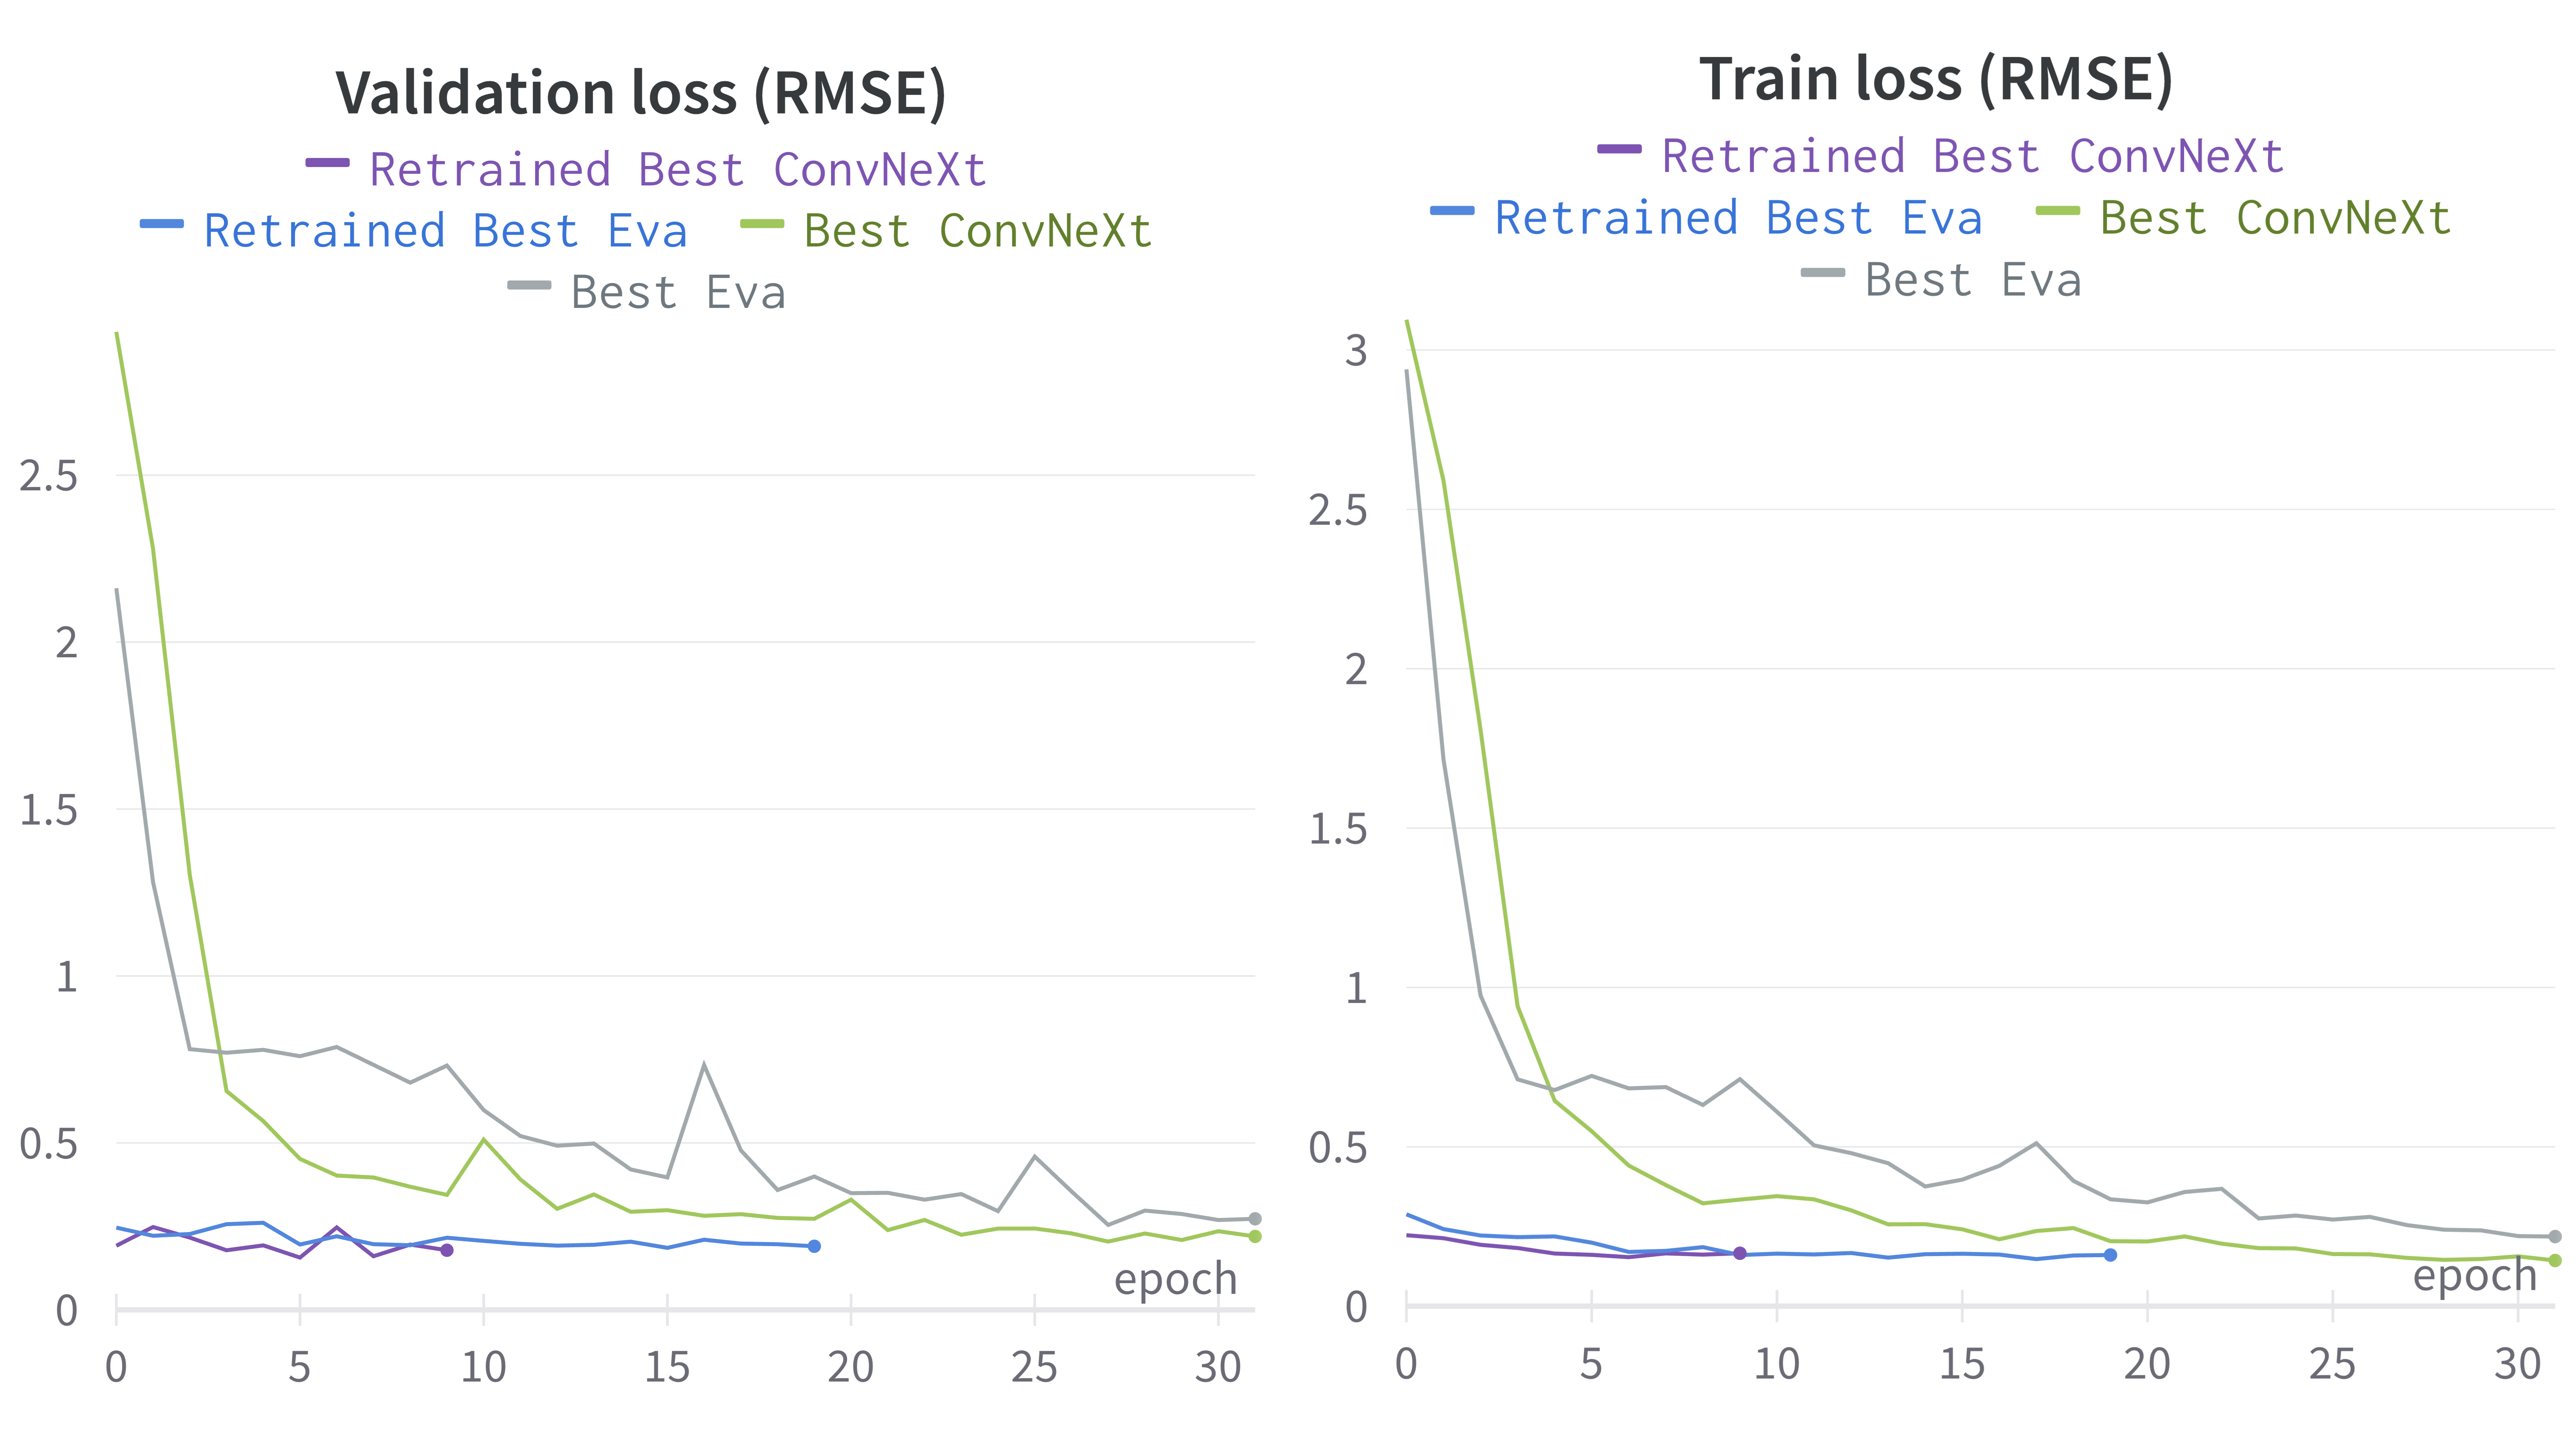
\includegraphics[trim={0cm 0cm 0cm 0cm},clip,width=1.0\textwidth]{images/train.png}
\caption{Training and validation loss for the best and retrained best frame-seqence-based competition models.}
\label{fig:training_validation_loss}
\end{figure}

As depicted in Figure~\ref{fig:training_validation_loss}, both the initial best and the retrained best models exhibit the expected trends in training and validation loss. Notably, the training loss for the retrained best models drops rapidly. This is anticipated since the retraining process targets the remaining portion of the data, thereby focusing on fine-tuning rather than learning from scratch.

\subsection{Retraining Gains}
During the competition, due to time constraints, our approach was to run the training script twice for each model—what we refer to as the 'double-run' method. To ensure that the results are directly comparable, we used the same random seed for frame-sequence sampling in both prediction runs.
\begin{table}[!htb]
\centering


\begin{tabular}{|c|c|c|c|c|}
\hline
Model & Test Set 1 & Test Set 2 & Test Set 3 & Final Score \\
\hline
Best ConvNeXt & 0.75 & 0.91 & 0.82 & 0.827 \\
\hline
Retrained Best ConvNeXt & 0.77 & 0.92 & 0.84 & 0.845 \\
\hline
Best Eva & 0.78 & 0.91 & 0.85 & 0.848 \\
\hline
Retrained Best Eva & 0.80 & 0.91 & 0.86 & 0.859 \\
\hline
\end{tabular}
\caption{Performance of Initial and Retrained Models}
\label{tab:retraining_gains}

\end{table}

Table \ref{tab:retraining_gains} indicates that retraining the models provided a boost in performance across all test sets, effectively raising the final scores. This suggests that our 'double-run' approach was not merely a workaround for tight deadlines but actually a method that contributed to optimizing the model's performance.


\section{Post-Competition Model Hyperparameter tunning}
After the competition, we had the chance to use the real labels and weren't limited by daily submission caps. This helped us do a deeper dive into fine-tuning our ConvNeXt model. We switched it to a frame-based setup, which improved its performance and made it easier to understand how it was making its predictions. We tweaked different settings during this stage and will go into the details of how this improved the model later on.

\subsection{Hyperparameter Optimization using Weights \& Biases Sweeps}
Weights \& Biases (WandB) Sweeps offer a structured and automated way to perform hyperparameter tuning. Through a single config file it enables automatic testing of various parameter combinations with multiple agents running the training loop. WandB collected performance data, simplifying the selection of optimal settings. For efficient testing, each model predicted the MOS of only the middle frame in each test video. This offered a balance between speed and accuracy.

Various parameters were tested to optimize the frame-based ConvNeXt model, as detailed below
\begin{itemize}
    \item \textbf{Augment Probability}: \{0.5, 0.9\}
    \item \textbf{Use Augmentation}: \{True, False\}
    \item \textbf{Batch Size}: \{1, 8\}
    \item \textbf{Drop Path Rate}: \{0, 0.1, 0.2\}
    \item \textbf{Dropout Rate}: \{0.1, 0.5\}
    \item \textbf{Loss Function}: \{RMSE, MAE\}
    \item \textbf{Max Epochs}: \{16, 32, 48\}
    \item \textbf{Random Seed}: \{-1, 1126\}
    \item \textbf{Sequence Length}: \{8, 16, 32\}
    \item \textbf{Weight Decay}: \{0.01, 0.1, 0.001\}
\end{itemize}

In the following subsections, we will present the findings of the hyperparameter tuning process, starting with the significance of the seed parameter.
\subsubsection{Seed Parameter}
As evidenced in Figure \ref{fig:SEED}, the parameter importance chart showcases the relationship between the seed value, validation loss, and the final score based on the middle frames. The chart supports our observations that deterministic seeding (same seed value) leads to comparable validation losses, mainly influenced by other parameters such as batch size. Meanwhile, the non-deterministic seed (-1) shows a wider range of validation losses. Despite these variances in validation loss, the final scores remained relatively consistent across both seeded and non-seeded approaches. It's also evident that other hyperparameters have a noticeable impact on the final score. 

\begin{figure}[H]
\centering
\includegraphics[trim={0cm 2cm 0cm 2cm},clip,width=1.0\textwidth]{images/W&B Chart 03_09_2023, 15_11_19.png}
\caption{Parameter Importance Chart: Relationship between Seed, Validation Loss, and Final Score from Middle Frames.}
\label{fig:SEED}
\end{figure}
For comparability all subsequent analyses will use a fixed seed of 1126.




\subsubsection{Batch Size}
The figure \ref{fig:BatchSize} below illustrates the strong relationship between batch size and both validation loss and final score from middle frame evaluations. Notably, batch size emerged as the most significant hyperparameter in our model's performance.

A larger batch size led to higher validation loss and, consequently, worse model performance. This may be attributed to the fact that larger batch sizes provide a more accurate estimate of the gradient. However, they also reduce the model's ability to escape local minima in the loss landscape, potentially leading to sub-optimal solutions. It's worth noting that the effective batch size was 4, as the training was distributed across 4 GPUs.






\begin{figure}[H]
\centering
\includegraphics[trim={1cm 2cm 1cm 2cm},clip,width=1.0\textwidth]{images/W&B Chart 03_09_2023, 16_16_33 (1).png}
\caption{Parameter Importance Chart: Relationship between Batch Size, Validation Loss, and Final Score from Middle Frames.}
\label{fig:BatchSize}
\end{figure}

\section{Final Predictions and Model Averaging}
In this section, we focus on the performance of the top-performing models identified in the previous chapters. We'll explore their predictive accuracy on test sets, investigate the potential benefits of model ensembles, and evaluate the consistency of the predictions.

\subsection{Test Set Predictions}
Here, we will present the test set performance of our best models.


\begin{table}[h]

\smallskip
\begin{center}
\begin{tabular}{ | c | c | c | c | c | c | }
\hline  
  \textbf{Model} & \textbf{Test Set} & \textbf{PLCC$^{\uparrow}$} & \textbf{SRCC$^{\uparrow}$} & \textbf{RMSE$^{\downarrow}$} &
  \textbf{Score$^{\uparrow}$}\\ 
\hline  
  \multirow{3}{*}{ConvNext} & 1 & 0.7899 & 0.7387 & 0.4545 & \multirow{3}{*}{0.843} \\
                            & 2 & 0.9279 & 0.9171 & 0.3492 & \\
                            & 3 & 0.8647 & 0.8211 & 0.4303 & \\
\hline
  \multirow{3}{*}{Eva} & 1 & \textbf{0.8585} & \textbf{0.7919} & \textbf{0.4128} & \multirow{3}{*}{0.858}
  \\ & 2 & 0.9158 & 0.9119 & 0.3622 & \\
   & 3 & 0.8726 & 0.8285 & 0.4132 & \\
\hline

  \multirow{3}{*}{Ensemble} & 1 & 0.8091 & 0.7633 & 0.4352 & \multirow{3}{*}{0.854} \\
                            & 2 & 0.9287 &
                            0.9197 & 0.3447  & \\
                            & 3 & 0.8746 & 0.8318& 0.4146 & \\
                            \hline
  \multirow{3}{*}{Post comp. ConvNext} & 1 & 0.8265 & 0.7907 & 0.4160 & \multirow{3}{*}{\textbf{0.867}} \\
                            & 2 & \textbf{0.9323} & \textbf{ 0.9234} & \textbf{0.3233}  & \\
                            & 3 & \textbf{ 0.8922} & \textbf{0.8382} & \textbf{0.3749} & \\
\hline  
\end{tabular}
\end{center}
\caption{Performance Metrics for Competition and Post Competition Model on each Test Set.}
\label{res_test}
\end{table}

Table \ref{res_test} provides an overview of the performance metrics for our selected models across multiple test sets. The Eva model performs best on Test Set 1 with a PLCC of \(0.8585\), while the Post-competition ConvNext model has the highest overall score of \(0.867\).



\subsection{Model Ensembles}

In Table \ref{res_test}, the competition ensemble model consisting of Eva and ConvNext performed slightly worse than Eva alone but better than just ConvNext. This was because Eva was given a smaller weight of 0.25 in the ensemble based on its initial test performance. The difference in performance between Eva and the ensemble was marginal. In a subsequent ensemble model, detailed in Table \ref{res_ensemble}, we combined Eva and the Post-competition ConvNext with equal weights of 0.5, which led to an improved overall performance score.
\begin{table}[h]

\smallskip
\begin{center}
\begin{tabular}{ | c | c | c | c | c | c | }
\hline  
  \textbf{Model} & \textbf{Test Set} & \textbf{PLCC$^{\uparrow}$} & \textbf{SRCC$^{\uparrow}$} & \textbf{RMSE$^{\downarrow}$} &
  \textbf{Score$^{\uparrow}$}\\ 

\hline

  \multirow{3}{*}{Ensemble} & 1 & 0.8091 & 0.7633 & 0.4352 & \multirow{3}{*}{0.854} \\
                            & 2 & 0.9287 &
                            0.9197 & 0.3447  & \\
                            & 3 & 0.8746 & 0.8318& 0.4146 & \\
                            \hline

  \multirow{3}{*}{Post comp. ConvNext} & 1 & 0.8265 & 0.7907 & 0.4160 & \multirow{3}{*}{0.867} \\
                            & 2 & \textbf{0.9323} &  \textbf{0.9234} & \textbf{0.3233}  & \\
                            & 3 &  0.8922 & 0.8382 & \textbf{0.3749} & \\
\hline  

  \multirow{3}{*}{Post comp. Ensemble} & 1 & \textbf{0.8372} & \textbf{0.8027} & \textbf{0.4037} & \multirow{3}{*}{\textbf{0.8714}} \\
                            & 2 &  0.9307 & 0.9231 & 0.3298  & \\
                            & 3 & \textbf{ 0.8922} & \textbf{0.8423} & 0.3782 & \\
\hline  
\end{tabular}
\end{center}
\caption{Performance Metrics for Competition and Post Competition Model Ensembles on each Test Set.}
\label{res_ensemble}
\end{table}
\newpage





\subsection{Consistency of Predictions}
The frame-based ConvNext model offers a detailed look into the evolution of Mean Opinion Score (MOS) predictions over time. Figure \ref{fig:MOS_changes} highlights a specific example where the MOS experiences significant fluctuations. Initially, the individual is looking away from the camera with their eyes directed downwards, showing noticeable artifacts around the eyes and specifically at the top right edge of the forehead. As the person turns to face the camera, these artifacts become less prominent, and even the teeth appear more realistic. However, this visual realism takes a hit when the individual starts speaking, resulting in blurring around the chin. Finally, the person looks away from the camera again, and artifacts become noticeable on the right side of the face where the digitally rendered face meets the real background. These rapid fluctuations in MOS indicate that human raters are likely to notice these significant changes in quality. Consequently, the overall visual realism of the video may be rated based on the lowest-quality frames, as these are the most noticeable and impactful to the viewer.



\begin{figure}[H]
\centering
\includegraphics[trim={0.5cm 0cm 20cm 0cm},clip,width=1.0\textwidth]{images/mos_time.png}
\caption{Plot showing changes in predicted MOS (blue line) and actual MOS (red line) over time, along with key frames that highlight these changes.}
\label{fig:MOS_changes}
\end{figure}

\newpage

\section{Competition Comparison}
In this section, we compare the performance of our models against those submitted in the competition. This serves as an external benchmark to gauge the effectiveness of the techniques and approaches used in our work. 
\begin{table}[h]

\smallskip
\begin{center}
\begin{tabular}{ | c | c | c | c | c |  }
\hline  
  \textbf{Model} & \textbf{Test Set} & \textbf{PLCC$^{\uparrow}$} & \textbf{SRCC$^{\uparrow}$} & 
  \textbf{Score$^{\uparrow}$}\\ 

\hline
  \multirow{3}{*}{OPDAI} & 1 & \textbf{0.8578} & \textbf{0.8372} &  \multirow{3}{*}{\textbf{0.8851 }} \\
                            & 2 &  \textbf{0.9423}& \textbf{0.9214} & \\
                            & 3 & \textbf{ 0.8928} & \textbf{0.8592} & \\
                             \hline
\multirow{3}{*}{HUST} & 1 & 0.8117 & 0.7864 &  \multirow{3}{*}{0.8611} \\
                            & 2 & 0.9281 &
                            0.9215  &  \\
                            & 3 & 0.8842 & 0.8348&  \\
                            \hline

  \multirow{3}{*}{Our Ensemble} & 1 & 0.8091 & 0.7633  & \multirow{3}{*}{0.854} \\
                            & 2 & 0.9287 &
                            0.9197 & \\
                            & 3 & 0.8746 & 0.8318&  \\
                            \hline

  \multirow{3}{*}{Organizer baseline\cite{sun2023visual}} & 1 & 0.3778 & 0.4731  & \multirow{3}{*}{0.5470} \\
    & 2 & 0.5949 &
    0.7322 & \\
    & 3 & 0.4898 & 0.6139 &  \\
    \hline




\end{tabular}
\end{center}
\caption{Performance Metrics for Competition and Post Competition Model Ensembles on each Test Set.}
\label{res_final}
\end{table}

As seen in Table \ref{res_final}, the first-place model, OPDAI, achieved the highest score of \(0.8851\) utilizing a Swin Transformer backbone along with Norm-in-Norm and KL Divergence loss. The second-place model, HUST, employed an ensemble of ConvNext and LSTM models and used a combination of MAE, rank, and PLCC losses to reach a score of \(0.8611\). Our Ensemble model follows closely behind with a score of \(0.854\). The Organizer's baseline model, constructed using SVR regression on features extracted by both Swin Transformer and ConvNeXt—both pretrained on deepfake detection—and employing MSE loss, significantly lags behind with a score of \(0.5470\).









\section{Examples and discussion}
In this section, we showcase examples of both accurate and inaccurate MOS (Mean Opinion Score) predictions made by our best-performing ensemble model. This model is an ensemble of Eva and the frame-based ConvNext. The figures below are arranged in grids where each cell represents a frame from the video test set, accompanied by its predicted and actual MOS values as well as its test set identifier.

As evidenced in Figure \ref{fig:badpred}, the ensemble model of Eva and frame-based ConvNext occasionally generates imprecise MOS predictions. These instances are sorted by MAE in descending order, with the most inaccurate at the top. Notably, a large portion of these incorrect predictions stem from Test Set 1. This set is ID-disjoint from the training data, meaning the faces in this set were not seen during training. The absence of a reference face in Test Set 1 complicates the model's task of assessing visual realism. In Test Set 2, where reference faces are available, the model can comparatively evaluate the discrepancies between the manipulated and the original faces. This relative comparison simplifies the task and usually leads to more accurate MOS predictions. In contrast, Test Set 1 forces the model to make absolute judgments on visual realism without a point of comparison, making it a more challenging evaluation environment and contributing to higher inaccuracies.

In contrast, Figure \ref{fig:goodpred} displays instances where the model's predictions are notably accurate. These are also sorted by MAE, but in ascending order to showcase the best predictions.

\begin{figure}[!htb]
\centering
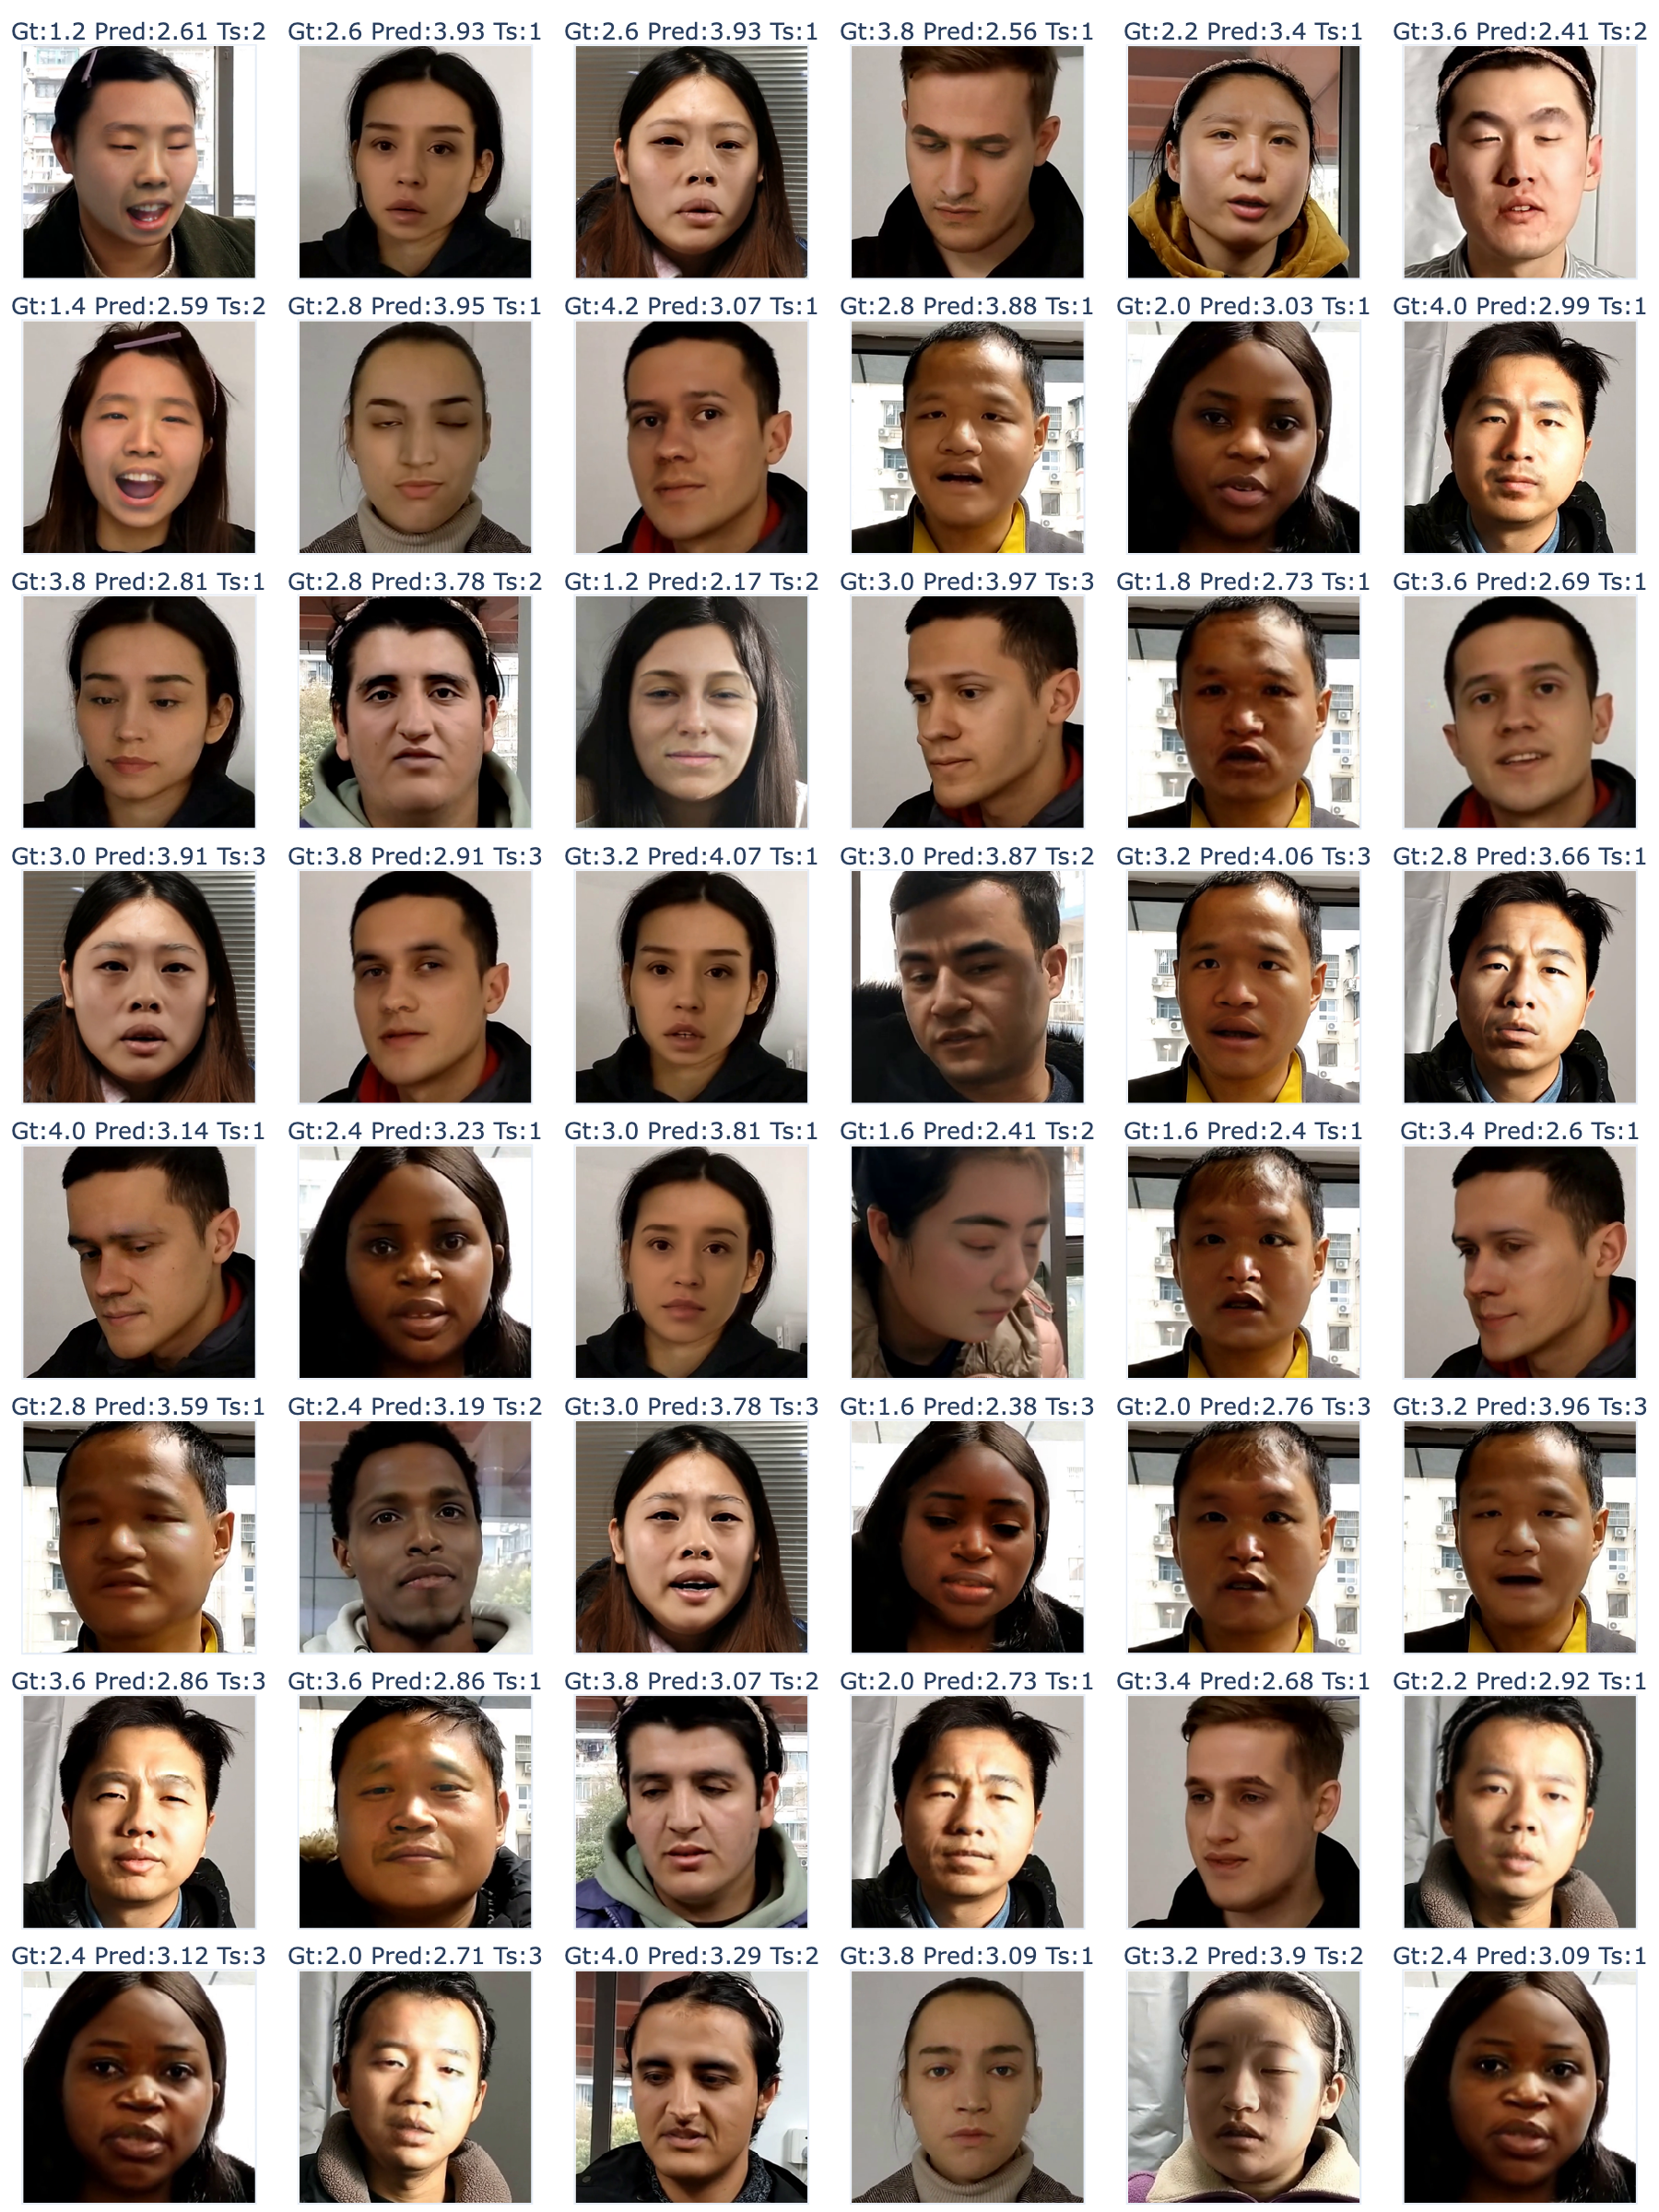
\includegraphics[trim={0cm 0cm 0cm 0cm},clip,width=1.1\textwidth]{images/badpred3.png}
\caption{Grid of frames showing most inaccurate MOS predictions (Pred), ground truth (Gt), and test set identifiers (Ts), sorted in descending order by MAE.}
\label{fig:badpred}
\end{figure}

\begin{figure}[!htb]
\centering
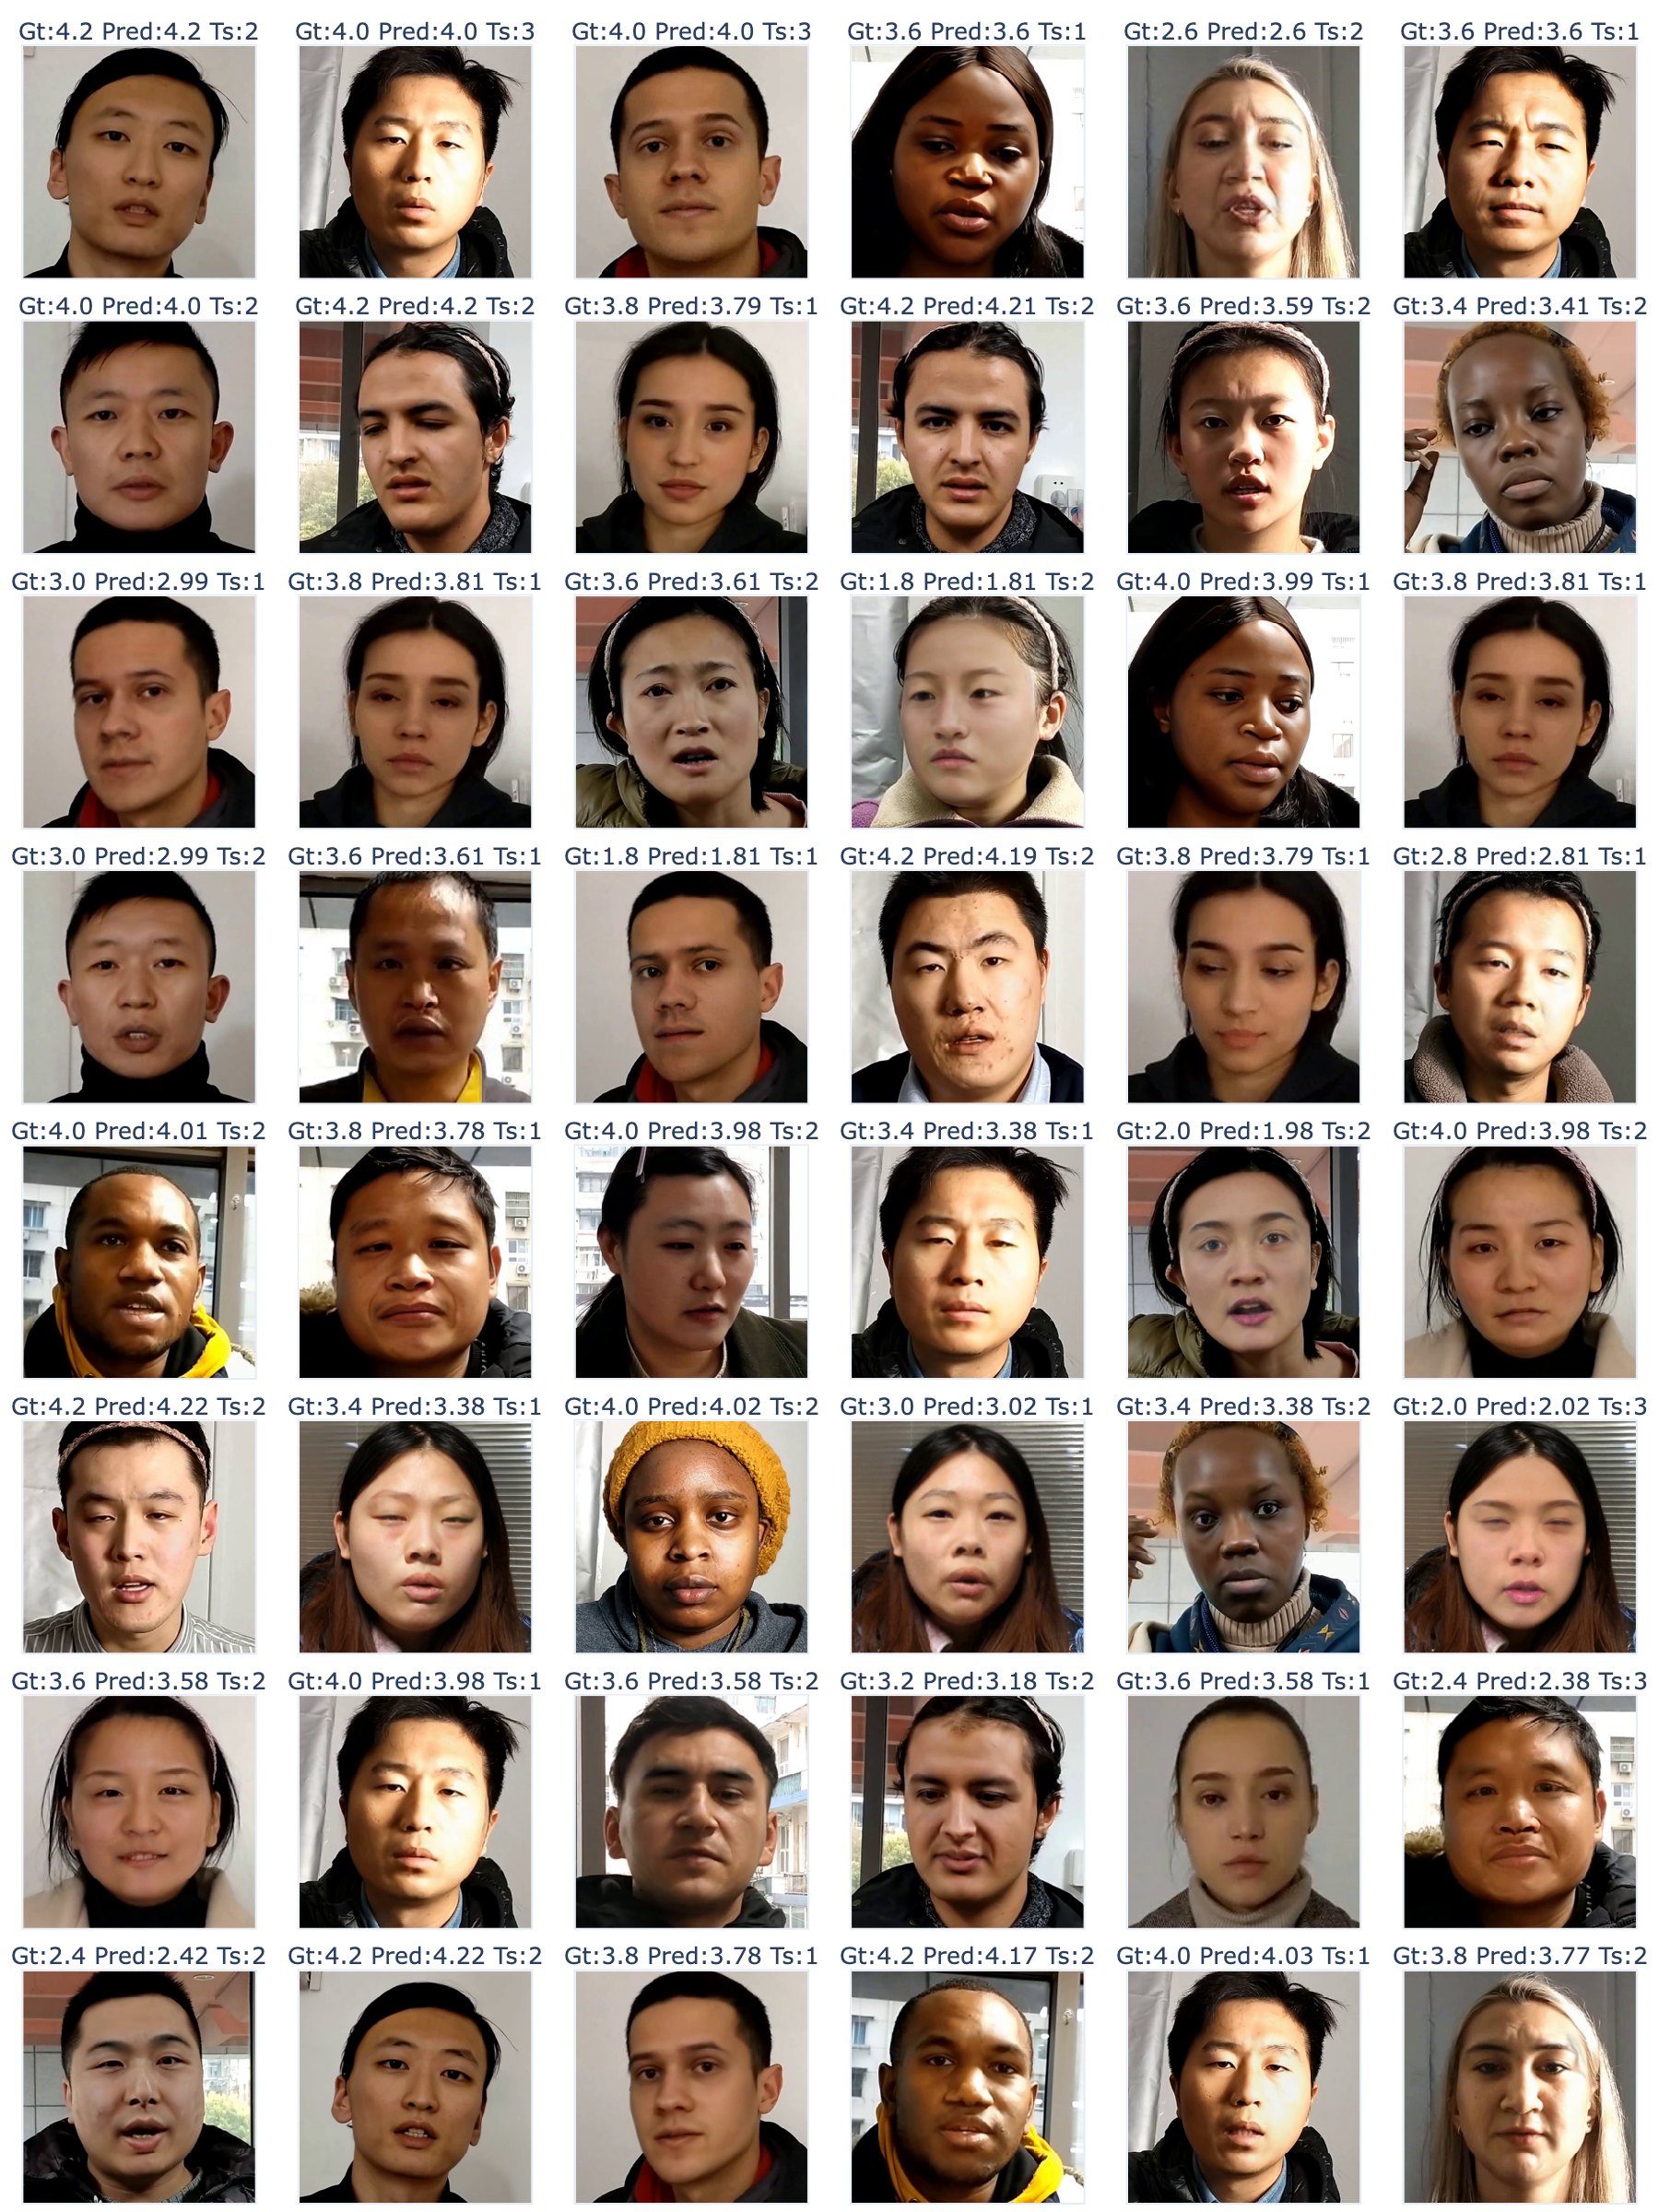
\includegraphics[trim={0cm 0cm 0cm 0cm},clip,width=1.1\textwidth]{images/goodpred.png}
\caption{Grid of frames showing most accurate MOS predictions (Pred), ground truth (Gt), and test set identifiers (Ts), sorted in ascending order by MAE.}
\label{fig:goodpred}
\end{figure}
\chapter{Conclusion}
 In conclusion, this thesis has successfully tackled the growing concerns surrounding DeepFake technology by introducing a robust method for assessing the visual realism of DeepFake videos.
 By harnessing the capabilities of ConvNext, a Convolutional Neural Network, in conjunction with Eva, a vanilla Vision Transformer (ViT), we've created an ensemble model that provides precise Mean Opinion Score (MOS) predictions. Notably, our approach has proven effective, earning us a third-place finish in the DeepFake Game Competition on Visual Realism Assessment (DFGC-VRA) 2023.
Beyond the accomplishments, our work also addresses several challenges inherent to the field. These include managing large video datasets needing strategic preprocesing, training large models in cluster enviroments on multiple GPUs and striking a balance beetwen models performance and the computational complexity required.
Overall, the success of this thesis underscores the untapped potential for further innovations in DeepFake detection and visual realism assessment, setting a benchmark for the next wave of research in this critical area of study.






\label{ch4}


%\cleardoublepage
%\addcontentsline{toc}{chapter}{Literatura}

% če imaš težave poravnati desni rob bibliografije, potem odkomentiraj spodnjo vrstico
\raggedright


\printbibliography[heading=bibintoc,type=article,title={Journal articles}]

\printbibliography[heading=bibintoc,type=inproceedings,title={Articles in Proceedings}]

\printbibliography[heading=bibintoc,type=incollection,title={Chapters in books}]

% v zadnji verziji diplomskega dela običajno združiš vse tri vrste referenc v en sam seznam in
% izpustiš delne sezname
\printbibliography[heading=bibintoc,title={Literature}]

\end{document}

